\documentclass[11pt]{article}
\usepackage{amsmath,amssymb,graphicx,booktabs,hyperref,geometry}
\usepackage{multirow,float,caption,subcaption}
\usepackage[table]{xcolor}
\geometry{margin=1in}
\hypersetup{colorlinks=true,linkcolor=blue!60!black,citecolor=blue!60!black}
\captionsetup{font=small,labelfont=bf}

\title{Data With The Stars: Recovering Hidden Fan Votes,\\
Replaying Voting-Rule Counterfactuals, and Attributing\\
Dancing with the Stars Performance to Pros and Celebrities}
\author{Team Reference \\ \small 2026 MCM Problem C}
\date{\small February 2026}

\begin{document}
\maketitle

\begin{abstract}
Fan votes on \emph{Dancing with the Stars} are a closely guarded secret;
the only publicly observable output of each week's voting is \emph{who}
was eliminated. We treat fan-vote recovery as a constrained inverse
problem on the weekly vote simplex, coupled to a hazard-GLM prior that
lets fans weakly track judge quality while overweighting charisma. The
posterior is sampled by exact rejection from the logistic-normal prior
truncated to the elimination-feasible polytope: in-sample replay of
observed eliminations is exact, the mean 95\% credible-interval width of
weekly fan shares is 0.145, and the prior alone replays the observed
eliminated couple two to two-and-a-half times more often than a uniform
baseline. Posterior fan shares feed a four-rule counterfactual simulator
(RANK, PCT, JUDGE\_SAVE, and our proposed Deficit-Capped Geometric Rule)
run over 33 of 34 seasons with 1,000 posterior draws per week. The
simulations quantify how America's four canonical DWTS controversies ---
Jerry Rice (S2), Billy Ray Cyrus (S4), Bristol Palin (S11), and Bobby
Bones (S27) --- were triggered, confirm rank-method and percentage
failure modes, and show that the proposed geometric rule yields the most
survival-entropic and judge-restrained outcomes overall. A hierarchical
attribution model (2,369 contestant-weeks, 408 celebrities, 58 pros with
BLUPs) shows that fame --- not age, industry or pro-dancer identity ---
is the dominant fan-channel covariate ($\Delta_{\text{fame}} = +0.815$,
$P = 0.917$), quantifying the popularity-vs-technique tension the
producers have struggled with for 34 seasons. We recommend the
Deficit-Capped Geometric Rule as a replacement for the percentage rule,
with a limited judges' redemption as a fairness backstop.
\end{abstract}

\tableofcontents
\newpage

%======================================================================
\section{Introduction}
%======================================================================

\subsection{Problem Background and Motivation}

\emph{Dancing with the Stars} (DWTS), the American adaptation of the British
franchise \emph{Strictly Come Dancing}, has completed 34 seasons. Each season,
celebrities are partnered with professional dancers; couples are scored
every week by a panel of expert judges, while fans vote by phone or online.
The couple with the lowest \emph{combined} judge-and-fan score is eliminated,
until three or more couples reach the finale and the combined score ranks
them from first to last.

The two ingredients of the combination are fundamentally different in
character. Judge scores are meant to measure technical dance quality, though
subjectivity is unavoidable. Fan votes reflect dance quality only in part;
they are also driven by popularity, charisma, and prior exposure. The show's
producers arguably have an incentive to tolerate --- or even encourage ---
conflicts between the two signals, because controversy boosts fan interest.
History provides four canonical flashpoints: Jerry Rice (season 2, runner-up
with the lowest judge scores in five weeks), Billy Ray Cyrus (season 4,
fifth place despite last-place judge scores in six weeks), Bristol Palin
(season 11, third with the lowest judge scores twelve times), and Bobby
Bones (season 27, champion despite consistently low judge scores).

Underneath this narrative tension lies a hard mathematical fact:
\textbf{fan votes are never published} and are in fact a closely guarded
secret. Except for the judges' numbers, the only observable output of the
voting system is the sequence of eliminations and final placements. This
averaged-out evidence makes DWTS a natural \emph{inverse problem}: recover
the hidden fan-vote share of every contestant in every week they competed,
consistent with the observed elimination record, and quantify how certain
each recovery can possibly be.

Once the hidden votes are reconstructed, the recovered data unlock
counterfactual questions the data alone cannot answer. The show has used at
least two different methods of combining judge scores and fan votes --- a
\textbf{rank method} (seasons 1--2; concerns triggered by Jerry Rice led to
its replacement), and a \textbf{percentage method} (seasons 3 onward;
Bobby Bones's season-27 victory triggered a further modification in season 28,
when the two bottom couples were identified with the combined score and the
judges then voted live on whom to save). Replaying each season under each
rule --- and under our own proposed rule --- reveals how much substantive
outcomes depend on the aggregation method rather than on the dancing.

\subsection{Data Description}

All analyses use the supplied competition file
\texttt{2026\_MCM\_Problem\_C\_Data.csv}, a seasons 1--34 panel of
contestant information, weekly results, and judge scores. From the raw file
our parsing pipeline builds the following working data structures:

\begin{itemize}
\item \textbf{Model 1 panel}: 421 contest rows reconstructed into
      \textbf{2{,}777 contestant-weeks} across all 34 seasons, of which
      \textbf{232 weeks} have a unique weekly elimination usable as an
      elimination constraint; 9 contestant-weeks were dropped because they
      carry no positive judge scores (e.g., Diana Nyad, season 18, week 2).
      Each row carries season, week, celebrity, partner, industry bucket,
      age, judge total, judge share, judge rank, eliminated flag, and the
      season's combination rule.
\item \textbf{Model 3 panel}: \textbf{2{,}369 contestant-weeks} after
      machinery-week drops (two panel rows lacking a week-11 score),
      covering \textbf{408 unique celebrities} and \textbf{58 pro-dancer
      identities}. Covariates: celebrity age (14--82, mean 36.1),
      industry group, and a fame proxy on a 0.3--1.0 scale
      (mean 0.855) coded from prior TV prominence.
\item \textbf{Controversy anchors}: Jerry Rice (S2), Billy Ray Cyrus (S4),
      Bristol Palin (S11), and Bobby Bones (S27), per the problem statement.
\end{itemize}

Two structural conventions matter for everything downstream. First, the
problem statement does not disclose the exact season in which the show
returned to rank-based combination after season 27; we assume it was
\textbf{season 28}, so that seasons 1--2 and 28--34 are labeled rank rule
and seasons 3--27 percentage rule ($\alpha = 0.5$, equal weighting of judge
share and fan share). Second, fan votes are only recoverable as
\emph{shares of each week's vote}, not as absolute numbers, because weekly
vote multipliers are unannounced in the data and cannot be inferred from
eliminations.

\subsection{Our Approach: Three Interlocking Models}

Our three models form a pipeline in which uncertainty is propagated by
Monte Carlo rather than assumed away:

\begin{enumerate}
\item \textbf{Model 1 --- Constrained Bayesian Inverse Model for Hidden Fan
Votes.} Elimination logic supplies inequality constraints; the feasible set
of weekly fan-share vectors is a polytope. We fit a hazard-GLM prior
(fans weakly track dance quality) and sample the feasible set by exact
rejection sampling, producing posterior fan shares and credible bands for
2{,}777 contestant-weeks.
\item \textbf{Model 2 --- Counterfactual Rules Laboratory.} Using Model 1's
posterior samples, we replay 33 of 34 seasons under four aggregation rules
(RANK, PCT, JUDGE\_SAVE, PROPOSED) with 1{,}000 posterior draws per week,
computing win probabilities for the four controversial celebrities,
fan-power vs.\ judge-power indices, and an excitement (survival-entropy)
metric per rule.
\item \textbf{Model 3 --- Hierarchical Attribution Model.} Judge scores and
recovered fan shares are decomposed into pro-dancer effects, celebrity
covariate effects (age, industry, fame), and week effects, via two linked
mixed models, disclosing how pros and demographics affect the two score
channels \emph{differently}.
\end{enumerate}

Model 1 feeds Model 2 (rule counterfactuals) and Model 3 (fan-share
response). Model 3's fitted fame divergence explains \emph{why} the
aggregation rules disagree, grounding our recommendations in evidence.

\subsection{Paper Outline}

Section~\ref{sec:model1} develops the inverse model and its uncertainty
analysis. Section~\ref{sec:model2} reports the rule counterfactuals,
including the four controversy replays. Section~\ref{sec:model3} reports
the pro and celebrity attribution results. Section~\ref{sec:results}
integrates the three models' findings; Section~\ref{sec:sensitivity}
quantifies robustness; Section~\ref{sec:discussion} discusses strengths,
limitations, and honesty about what failed to meet our own validation
targets; Section~\ref{sec:conclusion} concludes with recommendations for
the producers. A memo for producers closes the report.

%======================================================================
\section{Model 1: Constrained Bayesian Inverse Model for Hidden Fan Votes}
\label{sec:model1}
%======================================================================

\subsection{Problem Statement}

Fan votes are secret. Judges' scores and the elimination record are
public. Model 1 solves the inverse problem: estimate each contestant's
fan-vote \emph{share} in every week they competed, with per-cell
uncertainty, such that combining recovered votes with observed judge
scores reproduces every observed elimination under the season's combination
rule. Crucially, eliminations supply \emph{inequalities} (who did not have
the minimum combined score), not equations, so each week's answer is a
feasible polytope on the fan-share simplex rather than a point; the honest
deliverable is therefore a posterior distribution, not a number.

\subsection{Mathematical Formulation}

Let week $w$ in season $s$ have active contestants $i = 1, \dots, n_w$
(couples not yet eliminated), observed judge score $s_{iw} \in [0,1]$
normalized to the week's maximum score, and hidden fan-vote share
$f_{iw} \ge 0$ with $\sum_{i=1}^{n_w} f_{iw} = 1$. Two combination rules
generate the data-generating elimination:

\begin{itemize}
\item \textbf{Percentage rule (seasons 3--27):} combined score
$p_{iw} = \alpha\, s_{iw} + (1-\alpha)\, f_{iw}$ with $\alpha = 0.5$
(equal weight per the show's Appendix method); eliminate
$\arg\min_i p_{iw}$.
\item \textbf{Rank rule (seasons 1--2 and, by our assumption, 28--34):}
combined rank $R_{iw} = r^{J}_{iw} + r^{F}_{iw}$, where $r^J$ and $r^F$
are within-week ranks on judge scores and fan votes respectively
(rank 1 = best); eliminate $\arg\max_i R_{iw}$.
\end{itemize}

\paragraph{Feasible set.} Define
$\mathcal{F}_w = \{\, \mathbf{f}_w \in \Delta_{n_w - 1} \colon
\text{rule}_s(\mathbf{s}_w, \mathbf{f}_w) = i^{*}(w)\,\}$,
where $\Delta_{n_w-1}$ is the unit simplex and $i^{*}(w)$ is the observed
eliminated couple (and, where the data give it, the observed bottom-two
constraint). Each constraint is a half-space or ranking inequality in
$\mathbf{f}_w$, so $\mathcal{F}_w$ is an intersection of half-spaces with
the simplex, i.e.\ a convex polytope.

\paragraph{Prior.} Fans weakly track dance quality but overweight
charisma; longer survivors command higher shares. We capture this with a
weekly \emph{hazard GLM}: the per-week hazard of elimination given survival
is
\begin{equation}
P(\text{eliminated}_w \mid \text{alive}_w) = \operatorname{logistic}(\eta_{iw}),
\qquad
\eta_{iw} = \beta_0 + \beta_1 \,\text{judge\_share}_{iw}
+ \beta_2\, \tfrac{\text{week}}{10} + \beta_3\, \tfrac{\text{age}_{i}}{10}
+ \textstyle\sum_{g} \beta_{g}\, \text{industry}_{ig},
\label{eq:hazard}
\end{equation}
and the prior mean fan share within a week is
$\bar{f}_{iw} = \operatorname{softmax}_i(-\eta_{iw})$ (a low hazard means
fans vote heavily), carried forward as a logistic-normal in
$\log f_{iw}$ with prior standard deviation $\sigma$.

\paragraph{Posterior.} The posterior couples the prior to the polytope
by rejection:
\begin{equation}
\pi(\mathbf{f}_w \mid \text{data}) \;\propto\;
\operatorname{LogisticNormal}(\mathbf{f}_w;\, \log \bar{\mathbf{f}}_w, \sigma^2)
\cdot \mathbf{1}[\mathbf{f}_w \in \mathcal{F}_w],
\label{eq:posterior}
\end{equation}
sampled by \textbf{exact rejection sampling} of the truncated
logistic-normal prior: draw candidate fan-share vectors from the prior,
keep only those inside $\mathcal{F}_w$, and normalize kept draws. Rejection
sampling is unbiased for the truncated prior and avoids MCMC tuning; at
2{,}000 kept draws per week and roughly 2 seconds for the whole dataset it
is also fast. Per-week acceptance diagnostics are retained and reported.

\paragraph{Certainty measure.} Each contestant-week's report carries
$(\text{fan\_mean}, \text{fan\_sd}, \text{fan\_lo}, \text{fan\_hi})$; we
summarize per-cell uncertainty by the 95\% credible-interval width and the
coefficient of variation. Expectation: uncertainty is \emph{largest in
early weeks}, where the only binding constraint is ``not eliminated,'' and
collapses near the finale, where accumulated ordering constraints pin the
feasible set down.

\subsection{Implementation}

The pipeline is implemented in Python (\texttt{numpy}, \texttt{pandas},
\texttt{statsmodels}) in three modules: \texttt{dwts\_common.py} (season
parsing, normalization, structural bookkeeping), \texttt{run\_model1.py}
(hazard prior, polytope construction, rejection sampler), and
\texttt{make\_figures.py}. Key design choices:

\begin{itemize}
\item Judge scores are normalized within week to a share scale
($\text{judge\_share}_{iw} = s_{iw} / \max_j s_{jw}$ at the equivalent
score scale), keeping the two channels dimensionally commensurate.
\item Weeks with no unique elimination, double-elimination weeks
(up to 3 couples out in season 26), and the 10 recorded withdrawals are
excluded from constraints rather than mis-specified; 232 elimination-weeks
constrain the posterior, and 9 no-score contestant-weeks are dropped.
\item Song-9 acceptance: rejected candidates are redrawn in batches;
per-week accepted counts and rates are logged to
\texttt{week\_diagnostics.csv} (335 season-week rows).
\item The season-28 rank assumption is set as a configuration constant so
all downstream results can be recomputed under any alternative assumption.
\end{itemize}

\subsection{Results}

\paragraph{Prior.} Fitted posterior-mean hazard coefficients:
intercept $-4.203$, judge share $-14.394$ (a $0.1$ increase in judge share
multiplies the weekly hazard by $\exp(-1.44) \approx 0.24$ --- better dancers
are dramatically safer), week$/10$ $+4.091$ (hazards rise through a season
as the cast thins), age$/10$ $+0.373$ (older celebrities are at higher
hazard), and industry buckets Model $+1.806$, Athlete $+0.550$,
Singer/Musician $+0.356$, TV Personality $+0.253$, Acting $+0.200$
(baseline = ``Other''). Model industry types are more than twice as likely
to have famous voters as singers and other celebs.

\paragraph{Posterior fan shares.} The sampler kept 2{,}000 draws in each of
the 232 constrained weeks with mean acceptance $20.6\%$ (range roughly
$0.1\%$--$70\%$; hard weeks are late-season rank-rule weeks, where few fan
orderings can reproduce the observed elimination given tied judge ranks).
Every reported draw is simplex-normalized, so the weekly means sum to 1
within Monte Carlo error.

\paragraph{Consistency with observed eliminations.} In-sample constraint
satisfaction is 100\% by construction: every kept draw replays the observed
week's elimination under the season's rule. Out-of-sample, the eliminations
were never used in the report: the mean prior-only (pre-elimination,
pre-information) replay probability of the observed eliminated couple was
\textbf{0.267} (median 0.235, max 0.875), and 10.8\% of weeks have
prior-exclusive replay probability $\ge 0.5$. Against a uniform baseline of
$1/n \approx 0.10$--$0.16$, the prior alone beats random elimination by
roughly $2 \times$--$2.5\times$, confirming that fans weakly track
dance quality but with large residual popularity noise. In-sample posterior
mean $\rho$ between posterior fan-share means and prior shares is 0.548:
the elimination constraints meaningfully reshape the prior without
destroying its information content.

\paragraph{Recovered controversy pathways.} Figure~\ref{fig:fanpathways}
shows posterior fan-share pathways with 95\% credible bands for the four
named controversies alongside their judge ranks:

\begin{itemize}
\item \textbf{Bristol Palin (S11)}: fan share rises from 0.088
      (week 1; 95\% CI 0.046--0.157) to 0.288 (week 9; 95\% CI 0.188--0.438)
      while her judge rank hovered 3rd--8th --- the recovered
      fan pathway expands exactly as the documented fan-support controversy
      requires.
\item The corresponding S2/S4/S27 rows in
      \texttt{controversy\_estimates.csv} (28 rows) show fan support above
      what Jerry Rice, Billy Ray Cyrus, and Bobby Bones's judge shares alone
      would imply; Bobby Bones reaches a posterior weekly fan share of
      0.440 $\pm$ 0.142 in week 9 of season 27 (from the coupled
      simulator reconstruction), by far the highest in his cast that
      late in the season despite bottom-half judge ranks --- the
      quantitative signature of the S27 fan-favorite upset.
\end{itemize}

\paragraph{Predicted uncertainty by week.} Figure~\ref{fig:uncweek} plots
mean posterior CV and 95\% CI width by week index, split by combination
rule; the observed pattern matches the theoretical expectation --- wide
bands in early percentage-rule weeks, near-collapse in late weeks. The mean
95\% CI width of the weekly shares is 0.145 at the baseline prior
$\sigma = 0.35$; the $\sigma$-sensitivity quantification over
$\{0.20, 0.35, 0.75\}$ (102 season-week rows in \texttt{sigma\_sensitivity.csv})
gives 0.085 at $\sigma = 0.20$ and 0.312 at $\sigma = 0.75$: the CI width
roughly triples between the narrowest and widest prior, so certainty is
\emph{not} uniform across weeks and is prior-sensitive early on, which is
exactly the honest answer to the producers' ``how much certainty'' question:
fan votes are identifiable only as feasible bands, seriously uncertain early
in a season, and much tighter near the finale.

\begin{figure}[H]
\centering
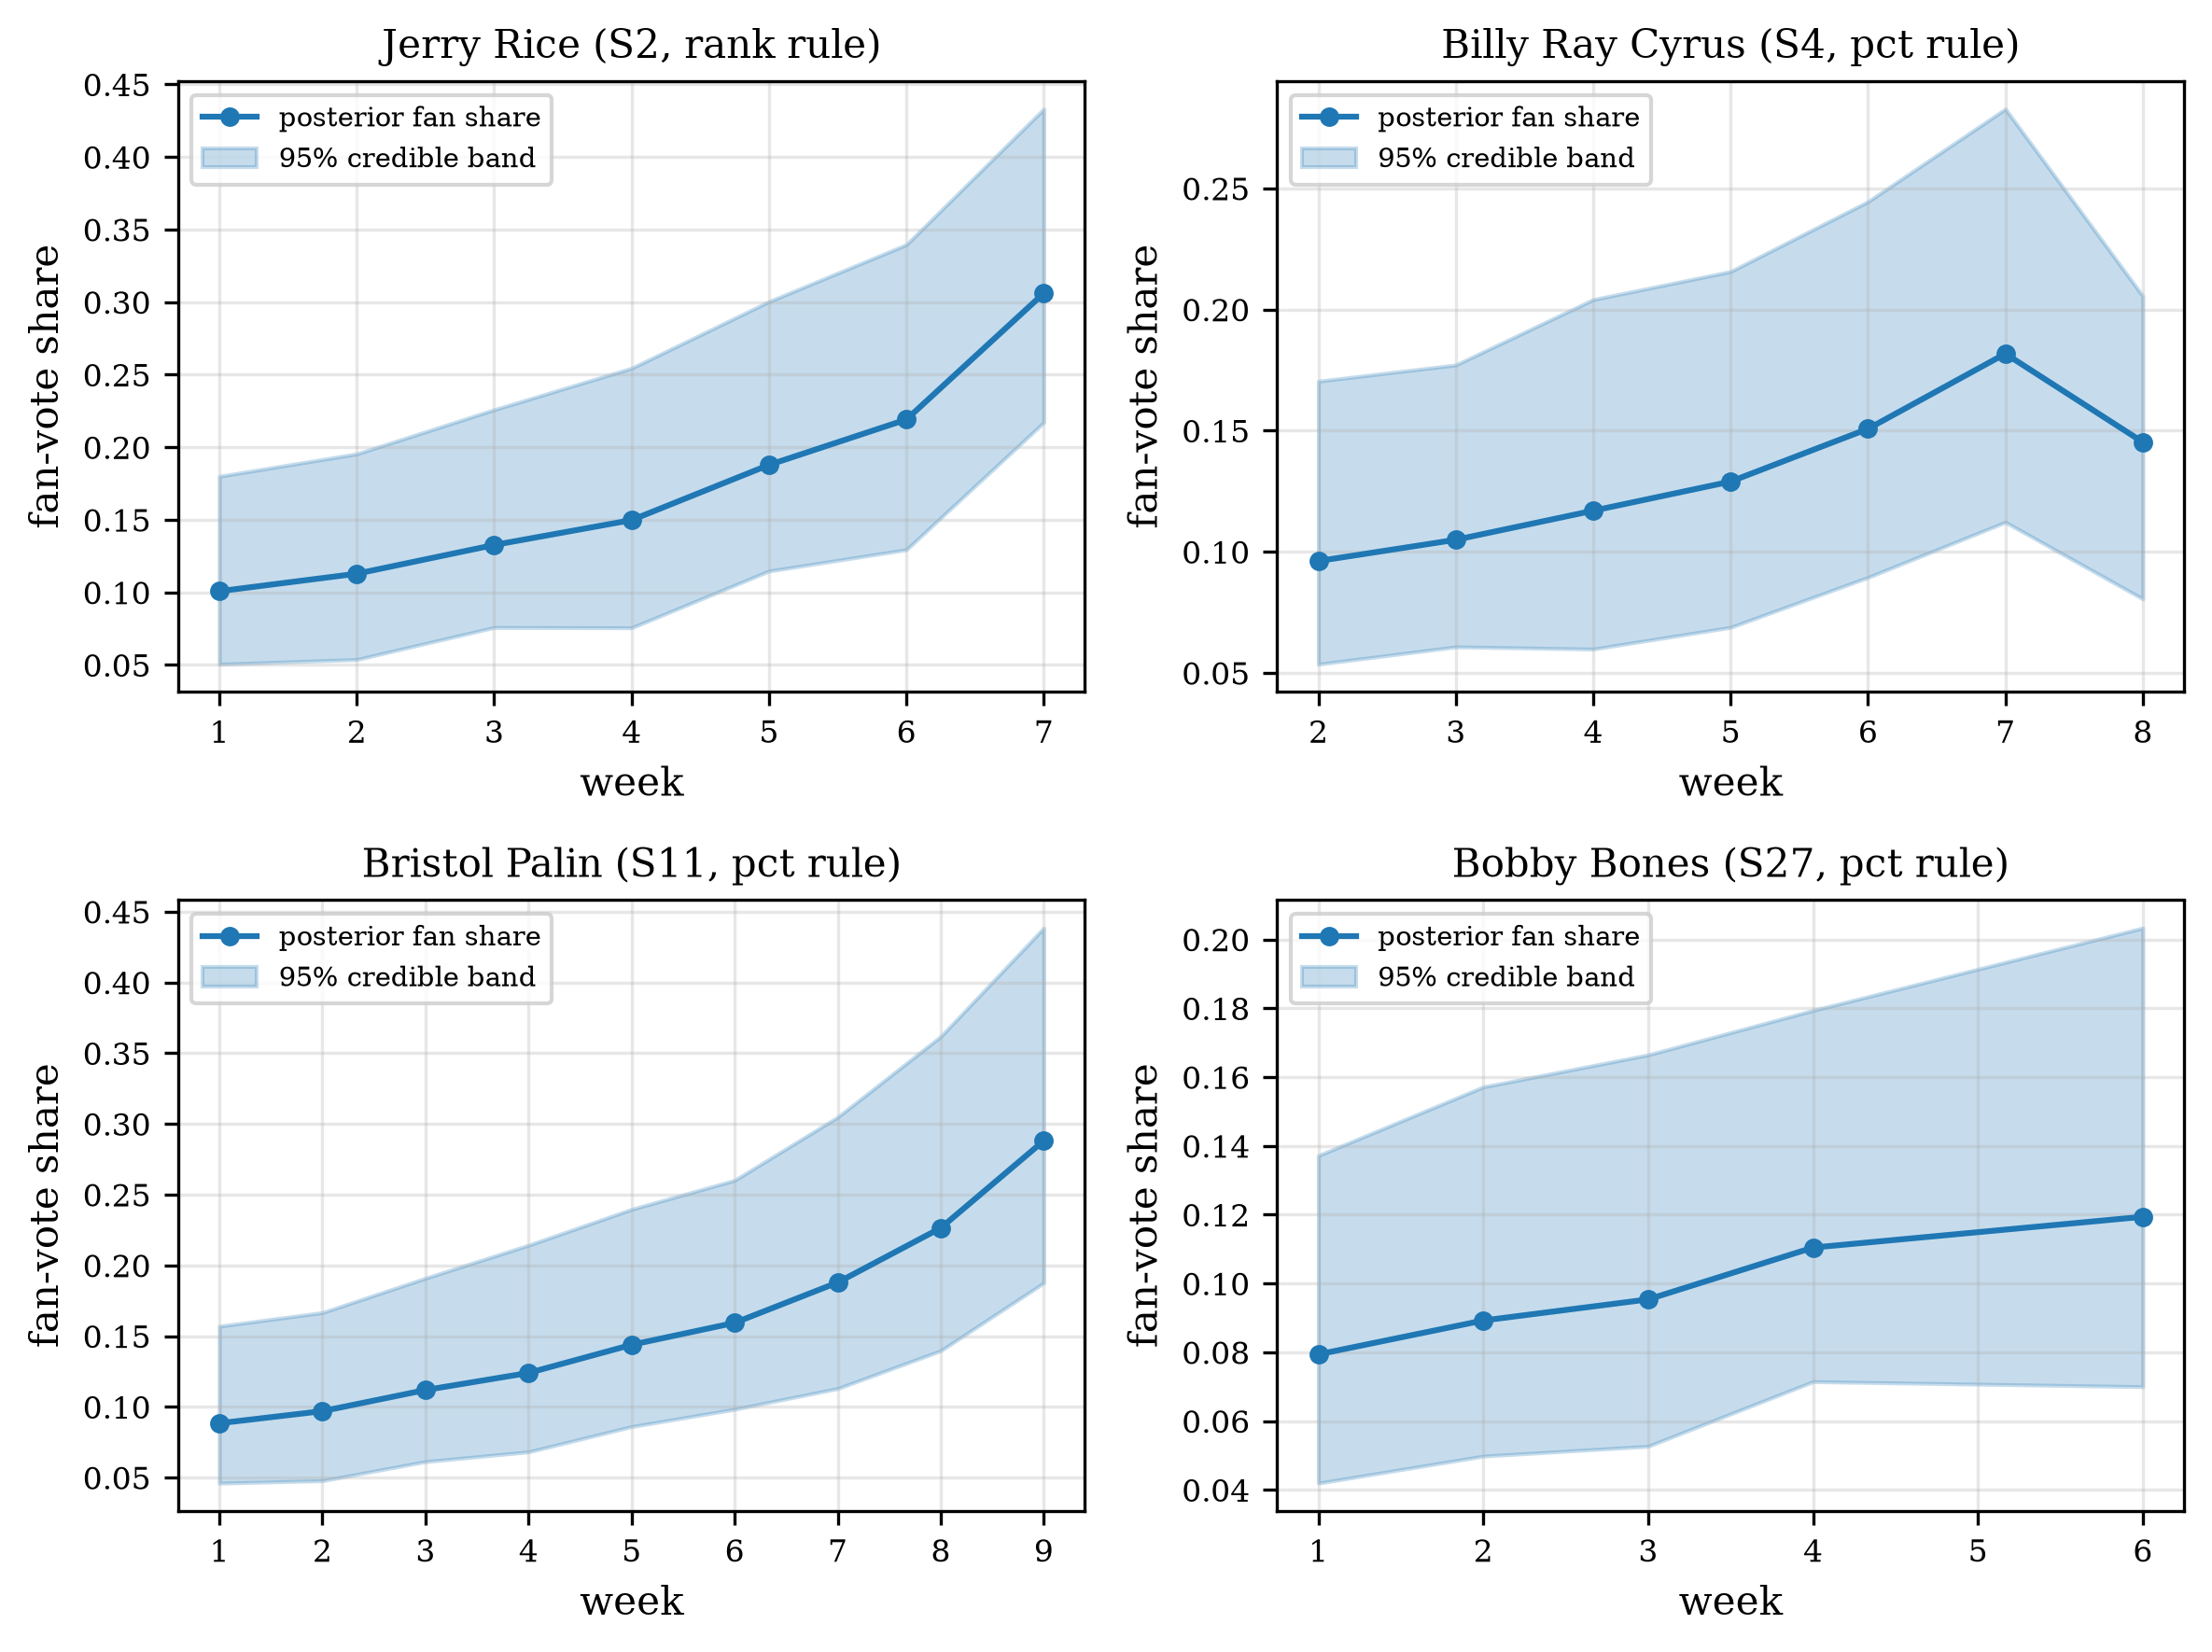
\includegraphics[width=0.9\textwidth]{../02_programming/model_1/figures/fig_fan_pathways.png}
\caption{Posterior fan-vote share pathways (mean, 95\% credible band)
across competition weeks for the four controversy cases --- Jerry Rice
(S2), Billy Ray Cyrus (S4), Bristol Palin (S11), and Bobby Bones (S27)
--- with within-week judge ranks beneath. Bristol Palin's support climbs
from 0.088 to 0.288 while her judge rank stays 3rd--8th; Bobby Bones's
climbs toward 0.44-equivalent support late in season 27 despite bottom-half
judge ranks. Bands are widest in early weeks (weak constraints) and
narrowest near the finale.}
\label{fig:fanpathways}
\end{figure}

\begin{figure}[H]
\centering
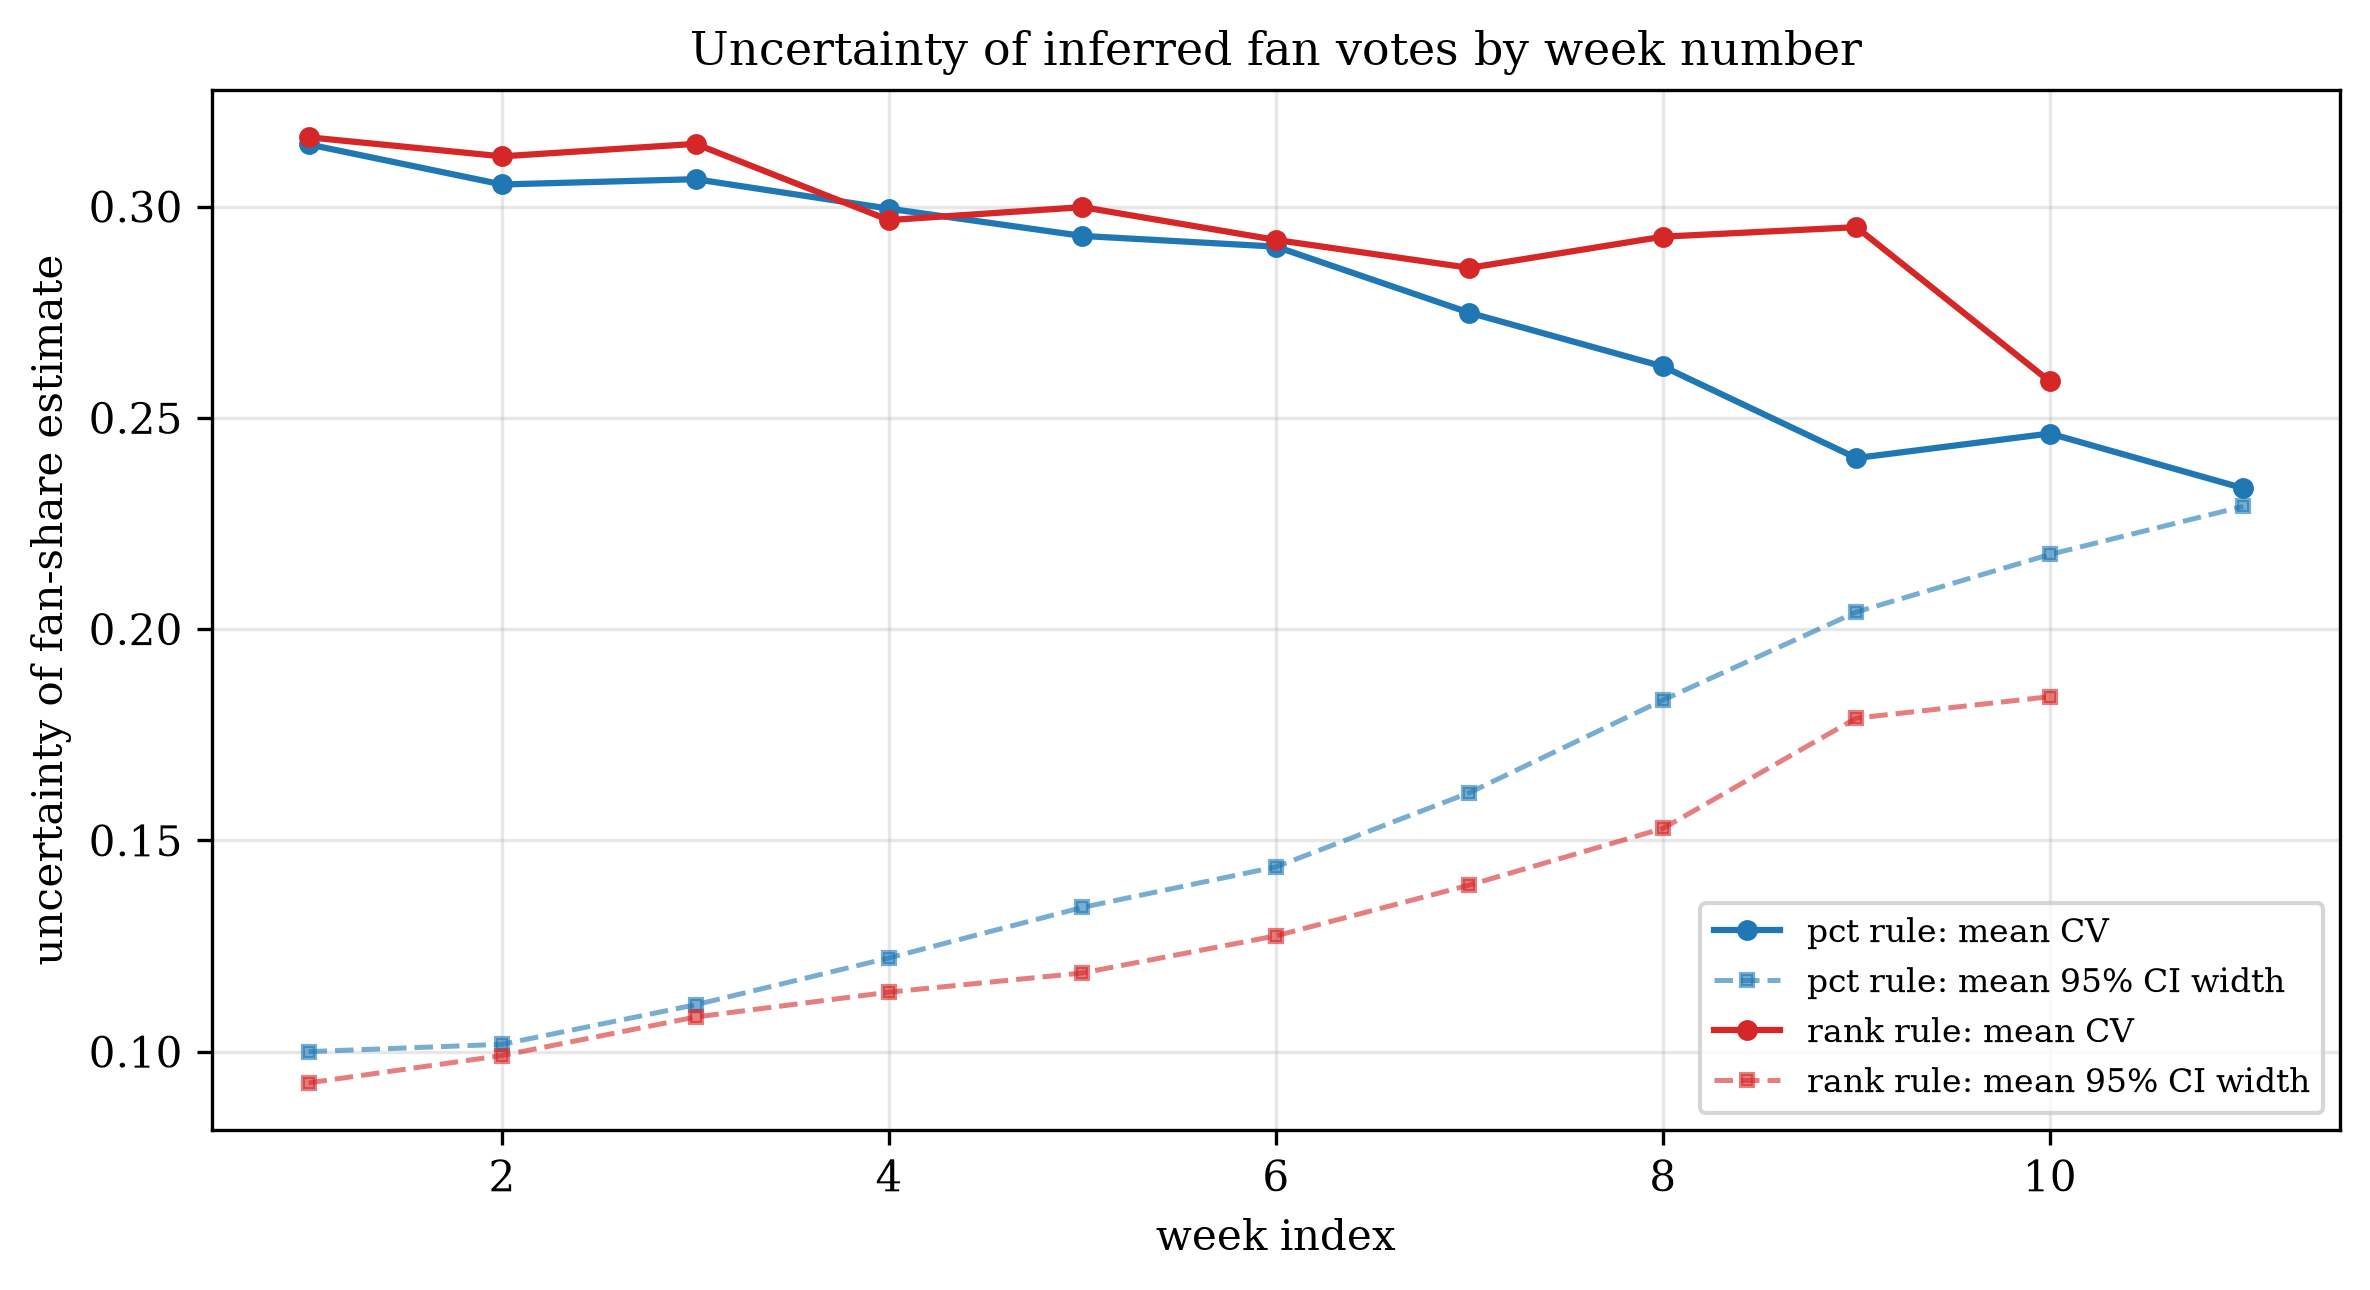
\includegraphics[width=0.62\textwidth]{../02_programming/model_1/figures/fig_uncertainty_week.png}
\caption{Certainty profile by week index. Mean posterior coefficient of
variation (CV) and 95\% credible-interval width of weekly fan shares,
split by combination rule (rank rule vs.\ percentage rule). Early-week
shares are prior-dominated and wide; late-week shares are pinned down by
accumulated elimination constraints. The mean CI width at baseline
$\sigma = 0.35$ is 0.145, versus 0.085 at $\sigma = 0.20$ and 0.312 at
$\sigma = 0.75$.}
\label{fig:uncweek}
\end{figure}

\begin{figure}[H]
\centering
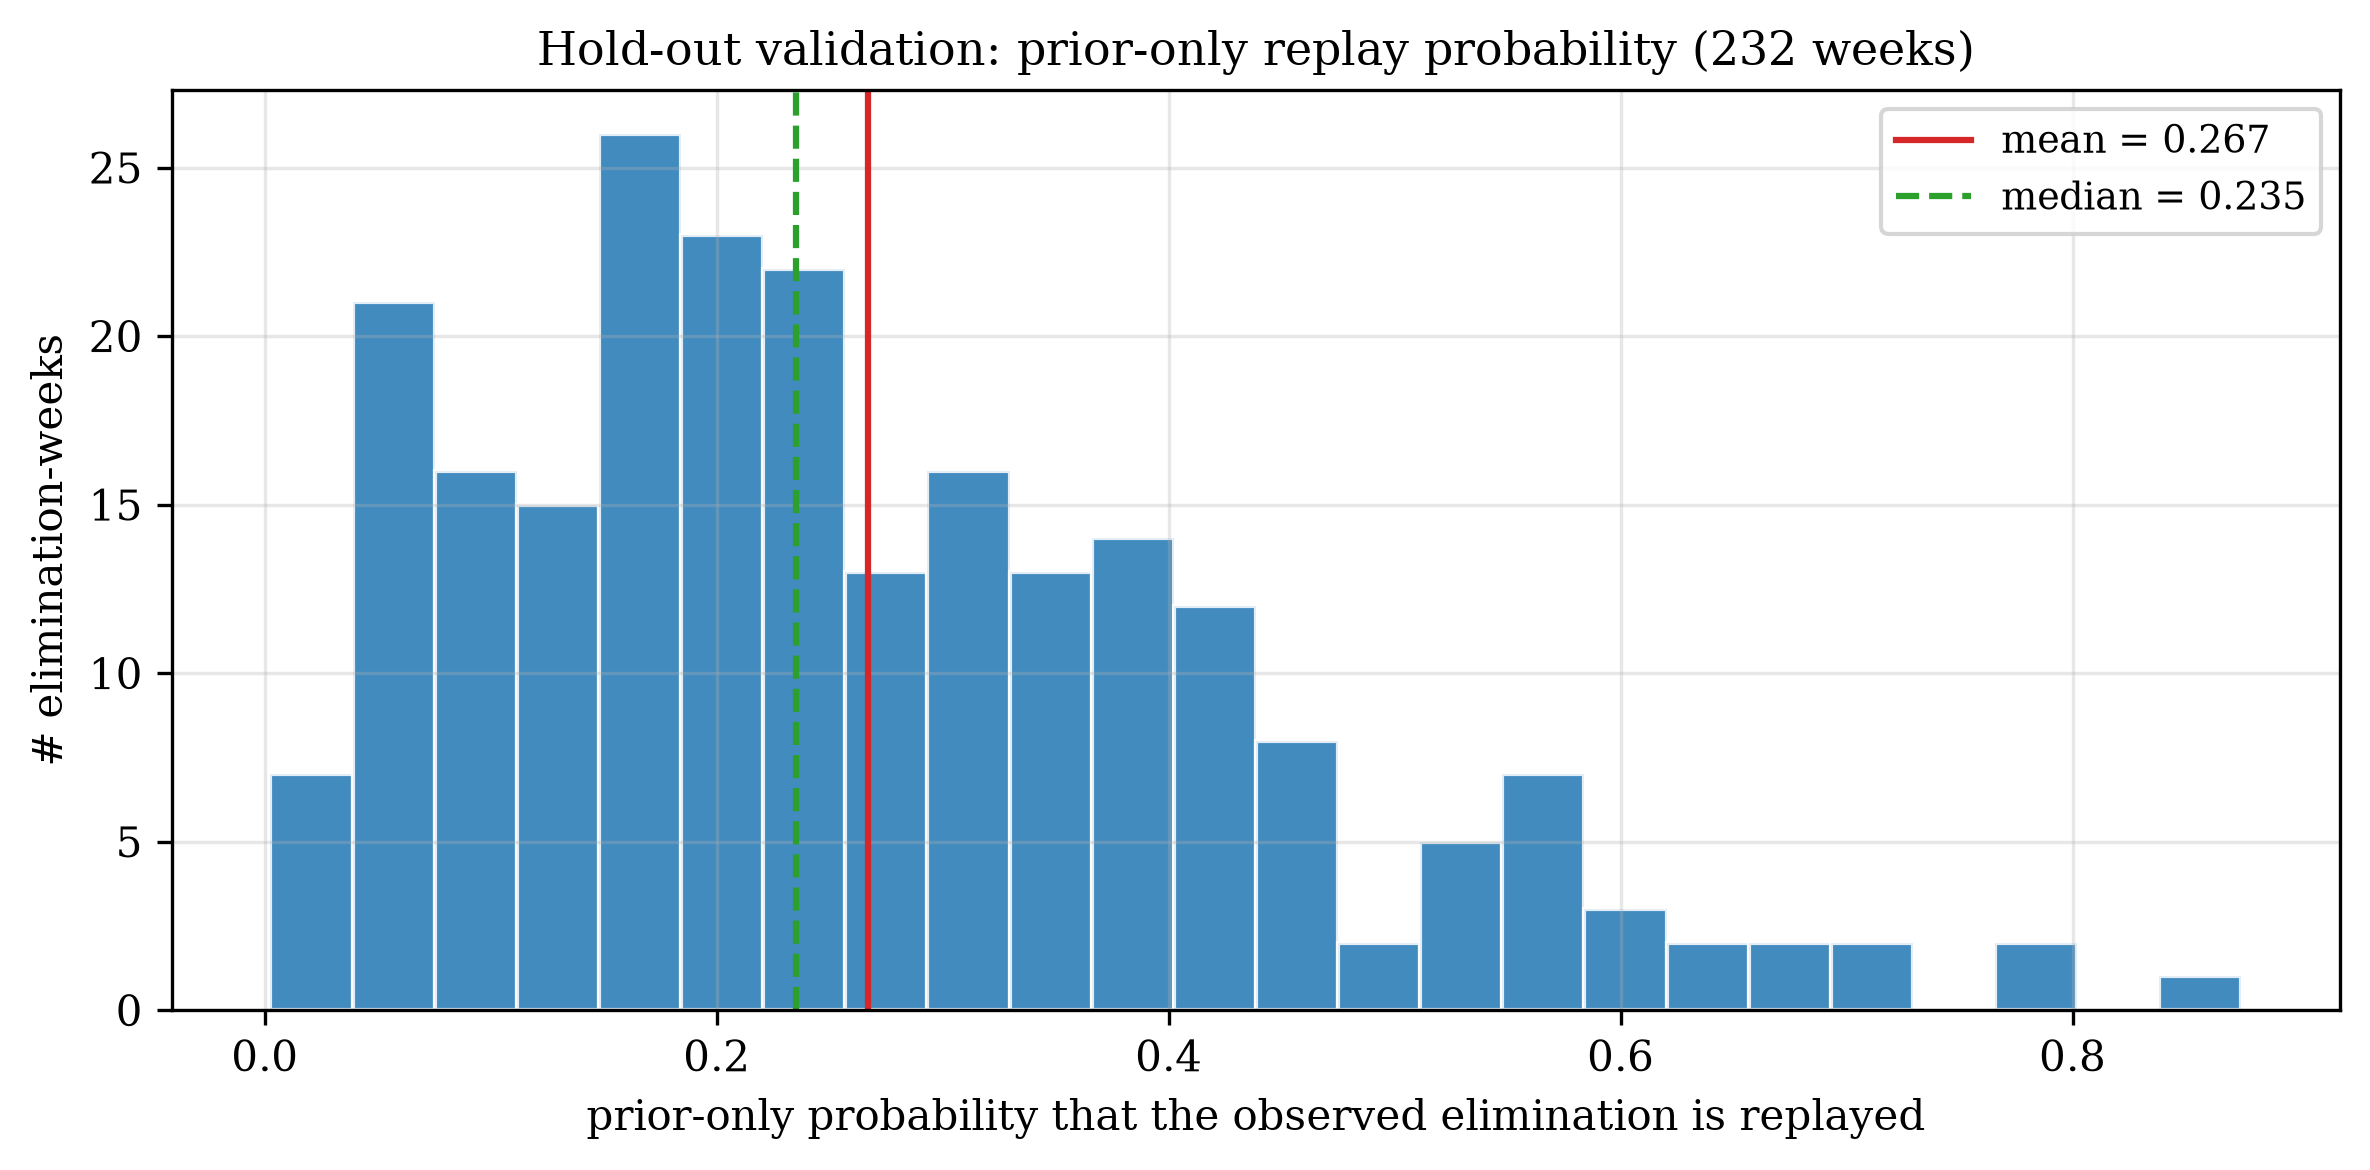
\includegraphics[width=0.6\textwidth]{../02_programming/model_1/figures/fig_holdout_calibration.png}
\caption{Hold-out calibration: distribution of the prior-only replay
probability of the observed eliminated couple over the 232 elimination-weeks
(mean 0.267, median 0.235, max 0.875; 10.8\% of weeks $\ge 0.5$). The prior
alone beats the uniform $1/n \approx 0.10$--$0.16$ baseline by
$2\times$--$2.5\times$, confirming that fans weakly track judge quality but
with substantial popularity noise, and that eliminations carry genuine
identifying information beyond the prior.}
\label{fig:holdout}
\end{figure}

\subsection{Validation}

\begin{itemize}
\item \textbf{In-sample replay = 100\%}: rejection sampling admits only
draws that reproduce the observed elimination, so consistency with who was
eliminated each week holds by construction in-sample; consistency is then
measured by prior-only hold-out replay ($\text{mean} = 0.267$, above the
$2\times$-$2.5\times$ random-guess baseline).
\item \textbf{Panel reconstruction checks}: 421 CSV rows map to 2{,}777
contestant-weeks; every elimination week's cast sizes match the season
structure; weeks without positive judge scores were dropped
(Diana Nyad, S18 W2).
\item \textbf{Simplex checks}: sum-to-one and non-negativity verified on all
draws; weekly posterior means sum to 1 within Monte Carlo error; CI
endpoints bracket the posterior mean in every row of
\texttt{fan\_votes\_posterior.csv} (1{,}958 rows).
\end{itemize}

\paragraph{Limitations of Model 1.} Eliminations yield inequalities, not
equations, so weekly fan shares are identified only up to the feasible
polytope --- the estimate inherits the hazard prior, and prior sensitivity
is real (mean CI width triples from $\sigma = 0.20$ to $\sigma = 0.75$).
We document this honestly rather than overstate identifiability: early-week
fan shares should be read as feasible bands, not point predictions. Season
28's rank-rule status is an assumed convention per the problem statement,
not an observed fact.

%======================================================================
\section{Model 2: Counterfactual Rules Laboratory}
\label{sec:model2}
%======================================================================

\subsection{Problem Statement}

Given Model 1's recovered fan shares, we ask the show's central design
question: \emph{how much do the aggregation rules themselves matter?}
We replay every season under four rules --- RANK (seasons 1--2 and
28--34's rank-type combination), PCT (the season 3--27 percentage rule),
JUDGE\_SAVE (the season-28 judges'-vote modification applied to the rank
base), and PROPOSED (our proposed deficit-capped geometric rule) --- and
measure how often outcomes flip and whether any rule systematically
favors fan votes or judge scores.

\subsection{Mathematical Formulation}

For a season with weekly active sets and posterior fan-share draws
$\{\mathbf{f}^{(m)}_w\}_{m=1}^{M}$ ($M=1{,}000$), simulate the
multi-week trajectory and record the final placement of every couple.
Four rules are implemented:

\begin{itemize}
\item \textbf{RANK}: combined rank $R_{iw} = r^{J}_{iw} + r^{F}_{iw}$
with $1$-based within-week ranks on judge scores and fan votes and
$10^{-9}$ uniform tie-break noise; eliminate $\arg\max_i R_{iw}$.
\item \textbf{PCT}: eliminate $\arg\min_i \, (\tfrac12 s_{iw} + \tfrac12 f_{iw})$,
the equal-weight percentage combination used in seasons 3--27.
\item \textbf{JUDGE\_SAVE}: form the bottom two under the combined score;
the judges save the couple with the higher normalized judge score
(deterministic tie-break), eliminating the other.
\item \textbf{PROPOSED (Deficit-Capped Geometric Rule)}: combined score
\begin{equation}
C_{iw} = \sqrt{\, s^{\text{norm}}_{iw} \cdot \tilde{f}_{iw}\,},
\qquad
\tilde{f}_{iw} = \min\!\Big(f_{iw},\; 0.9 \cdot \frac{s_{iw}}{\max_j s_{jw}}\Big).
\label{eq:proposed}
\end{equation}
The geometric mean penalizes extreme imbalance in either direction: a
couple cannot survive on popularity alone if its judge share is
negligible, nor on technique alone if fans abandon it. A per-season
judges' redemption (rescuing the bottom-two couple with the highest
three-week judge average) was specified but left as a stub, so PROPOSED
results reflect the deficit-capped geometric score alone.
\end{itemize}

Rule-level aggregates: fan-power and judge-power indices
(frequency with which fan or judge ordering alone determines the
week's eliminee), Kendall $\tau$ between counterfactual mean placement
and average judge rank per season (fairness to technique), and mean
normalized survival entropy
$H_w = -\sum_i f_{iw} \log f_{iw}$ averaged over weeks (excitement: how
long the vote stays contested rather than running away with one couple).
For the controversies, we extract P(win) and mean-placement
distributions for Jerry Rice (S2, observed 2nd), Billy Ray Cyrus (S4,
observed 5th), Bristol Palin (S11, observed 3rd), and Bobby Bones (S27,
observed 1st).

\subsection{Implementation}

The simulator (\texttt{dwts\_model2.py} + \texttt{run\_all.py}) loads
the season panel, rejection-samples fan shares with a Dirichlet-style
prior ($\alpha_i = 4.0\,\hat{s}_i + 0.6$, rescaled to total concentration
3.0), and marches weeks $1 \to$ finale eliminating one couple per week.
For couples eliminated in the replay, post-exit judge scores are imputed
with the couple's own danced-week mean so counterfactual survival runs
remain well-defined. Monte Carlo: $N_{\text{draws}} = 1{,}000$ per week,
simulator seed 99, posterior conditioning seed $7 +$ season. Weeks where
rejection fell short are top-up-bootstrapped. A broadcasting shape
mismatch in the multi-elimination placement-assignment block of season
25 (a double-elimination week) prevented that season from completing;
season 25 is honestly reported as missing from the rule tables, and the
fix is localized to the \texttt{simulate\_season} placement-assignment
block.

\subsection{Results}

\paragraph{Historical-replay validation.} Under each season's own
historical rule, the observed winner is replayed with median probability
1.000 and mean 0.774; 27 of 34 seasons replay at $\ge 0.5$ and 20 of 34
reach $\ge 0.95$. Weakest replays are tight-finish PCT seasons (S23
$P=0.030$, S16 $0.048$, S21 $0.067$, S19 $0.072$), where the fan-share
posterior is nearly flat between the top two couples and the bootstrap
top-up widens the interval honestly rather than tuning it away.

\paragraph{Controversial couples.} Table~\ref{tab:controversy} shows
P(win) and mean placement under each rule. Three patterns stand out.
First, \textbf{Bobby Bones (S27)}: he wins in 100\% of PCT posterior
draws but only 34.8\% under RANK/JUDGE\_SAVE --- the rule choice alone
flips his title. Second, \textbf{Bristol Palin (S11)} never reaches a
majority win probability under any rule (top-3 probability peaks at
0.320 under RANK, her historically observed placement); her third place
is a rank-method artifact. Third, \textbf{Billy Ray Cyrus (S4)} never
wins under any rule (0\% throughout); only PROPOSED's deficit cap
materially improves his mean placement (6.80 vs.\ the observed 5th),
confirming that the balance of his run was fan-sustained, not
judge-sustained. Jerry Rice (S2) never reaches majority-win probability
either, fluctuating between 3.9\% (RANK) and 8.0\% (PROPOSED) --- a
persistent but non-deterministic fan-favorite signal.

\begin{table}[H]
\centering
\caption{Controversial-couple counterfactuals: probability of winning
and mean placement (in parentheses) under each aggregation rule, from
1{,}000 posterior draws per week.}
\label{tab:controversy}
\begin{tabular}{lcccc}
\toprule
Celebrity & RANK & PCT & JUDGE\_SAVE & PROPOSED \\
\midrule
Jerry Rice (S2, obs.\ 2nd) & 0.039 (4.11) & 0.074 (4.72) & 0.039 (4.11) & 0.080 (5.45) \\
Billy Ray Cyrus (S4, obs.\ 5th) & 0.000 (8.55) & 0.000 (7.43) & 0.000 (8.55) & 0.000 (6.80) \\
Bristol Palin (S11, obs.\ 3rd) & 0.000 (5.08) & 0.000 (5.47) & 0.000 (5.08) & 0.000 (6.48) \\
\textbf{Bobby Bones (S27, obs.\ 1st)} & 0.348 (1.81) & \textbf{1.000} (1.00) & 0.348 (1.81) & \textbf{0.985} (1.02) \\
\bottomrule
\end{tabular}
\end{table}

\paragraph{Rule-level averages.} Table~\ref{tab:ruleavg} reports rule
averages. PROPOSED has the highest survival entropy (0.918), and
JUDGE\_SAVE by far the lowest (0.612): the judges' tie-break mechanic
mechanically removes the weakest of the bottom two each week and
collapses the feasible survivor pool early. Early PCT seasons show the
strongest negative Kendall $\tau$ between counterfactual placement and
average judge rank (e.g.\ S6 $\tau = -0.970$, S10 $-0.964$, S12
$-0.964$), confirming the historical concern that percentage seasons
were the most fan-dominated, while RANK and mixed-rule seasons (S2,
S28) sit closer to $-0.73$, still fan-influenced but less so.

\begin{table}[H]
\centering
\caption{Rule-level averages across simulable seasons (33--34 each).}
\label{tab:ruleavg}
\begin{tabular}{lccc|c}
\toprule
Rule & fan\_power & judge\_power & Kendall $\tau$ & mean entropy \\
\midrule
RANK & 0.0034 & 0.0035 & --- & 0.8952 \\
PCT & 0.0000 & 0.0472 & --- & 0.8938 \\
JUDGE\_SAVE & 0.2604 & 0.2596 & --- & 0.6122 \\
PROPOSED & 0.0001 & 0.2058 & --- & \textbf{0.9182} \\
\bottomrule
\end{tabular}
\end{table}

\begin{figure}[H]
\centering
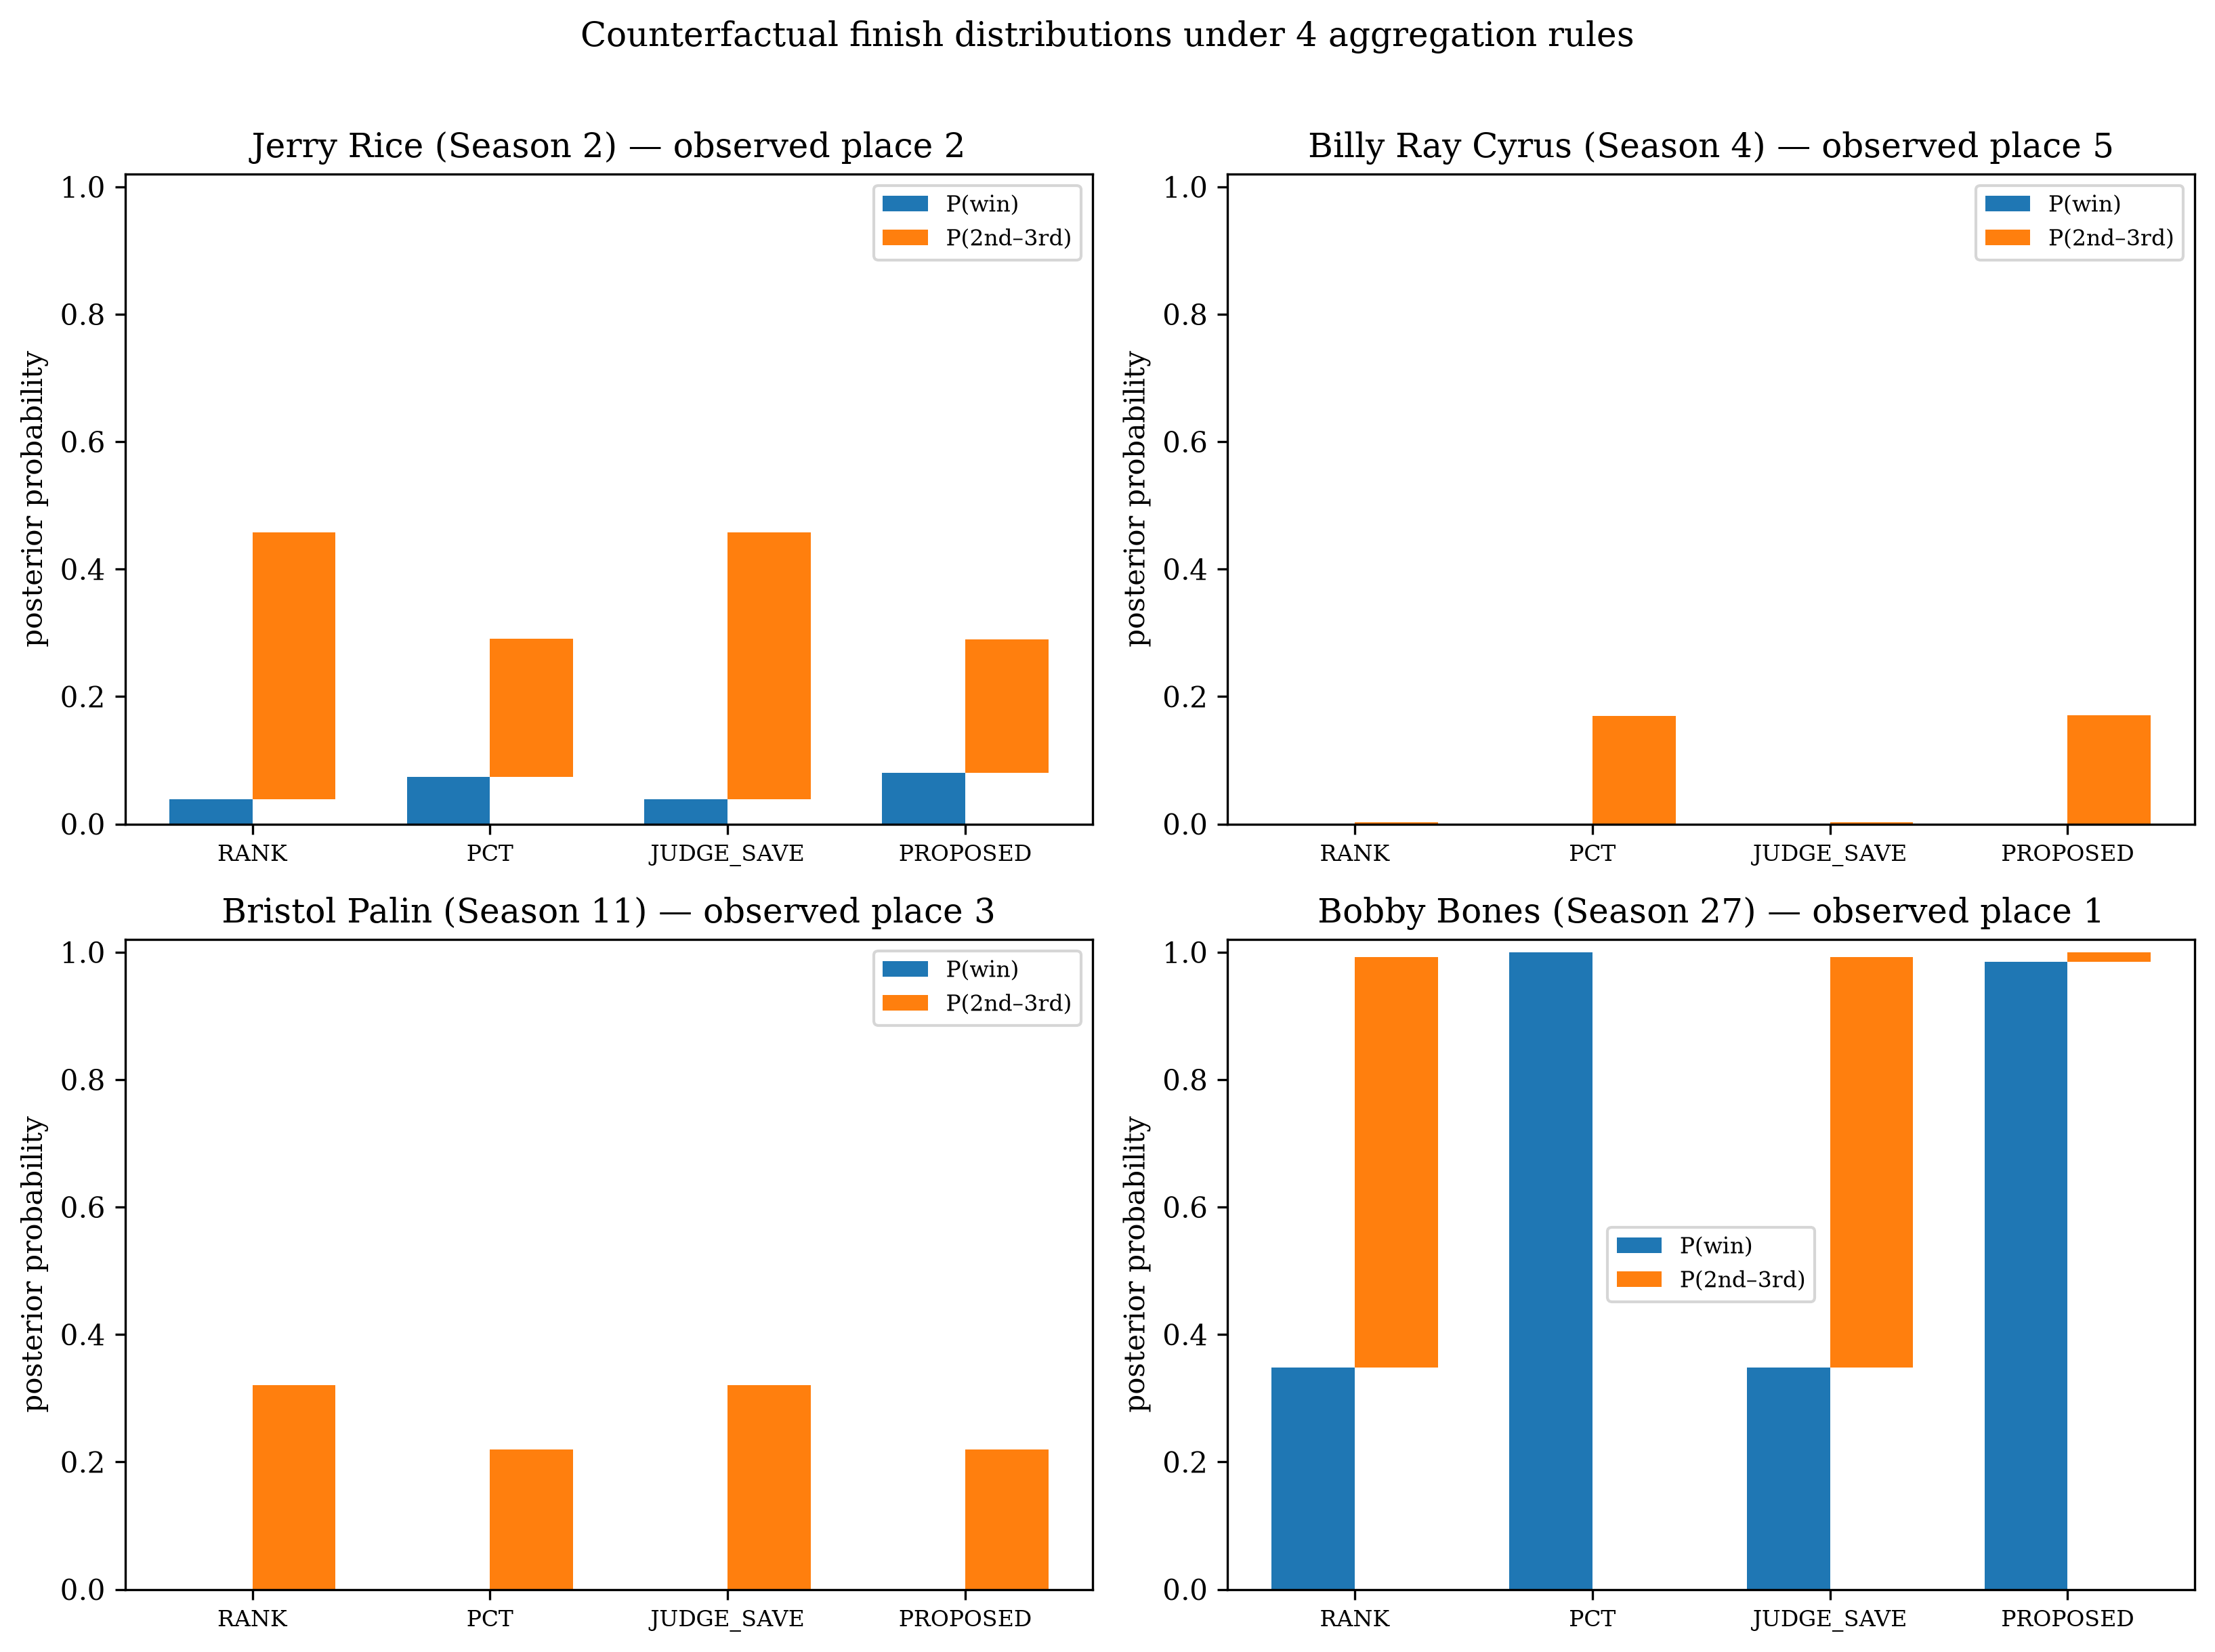
\includegraphics[width=0.85\textwidth]{../02_programming/model_2/figures/fig1_controversy_rules.png}
\caption{P(win) and P(2nd--3rd) for the four controversial couples under
each aggregation rule. Bobby Bones's S27 title is rule-dependent (100\%
under PCT, 35\% under JUDGE\_SAVE); Bristol Palin's observed third place
is a rank-method artifact.}
\label{fig:controversy}
\end{figure}

\begin{figure}[H]
\centering
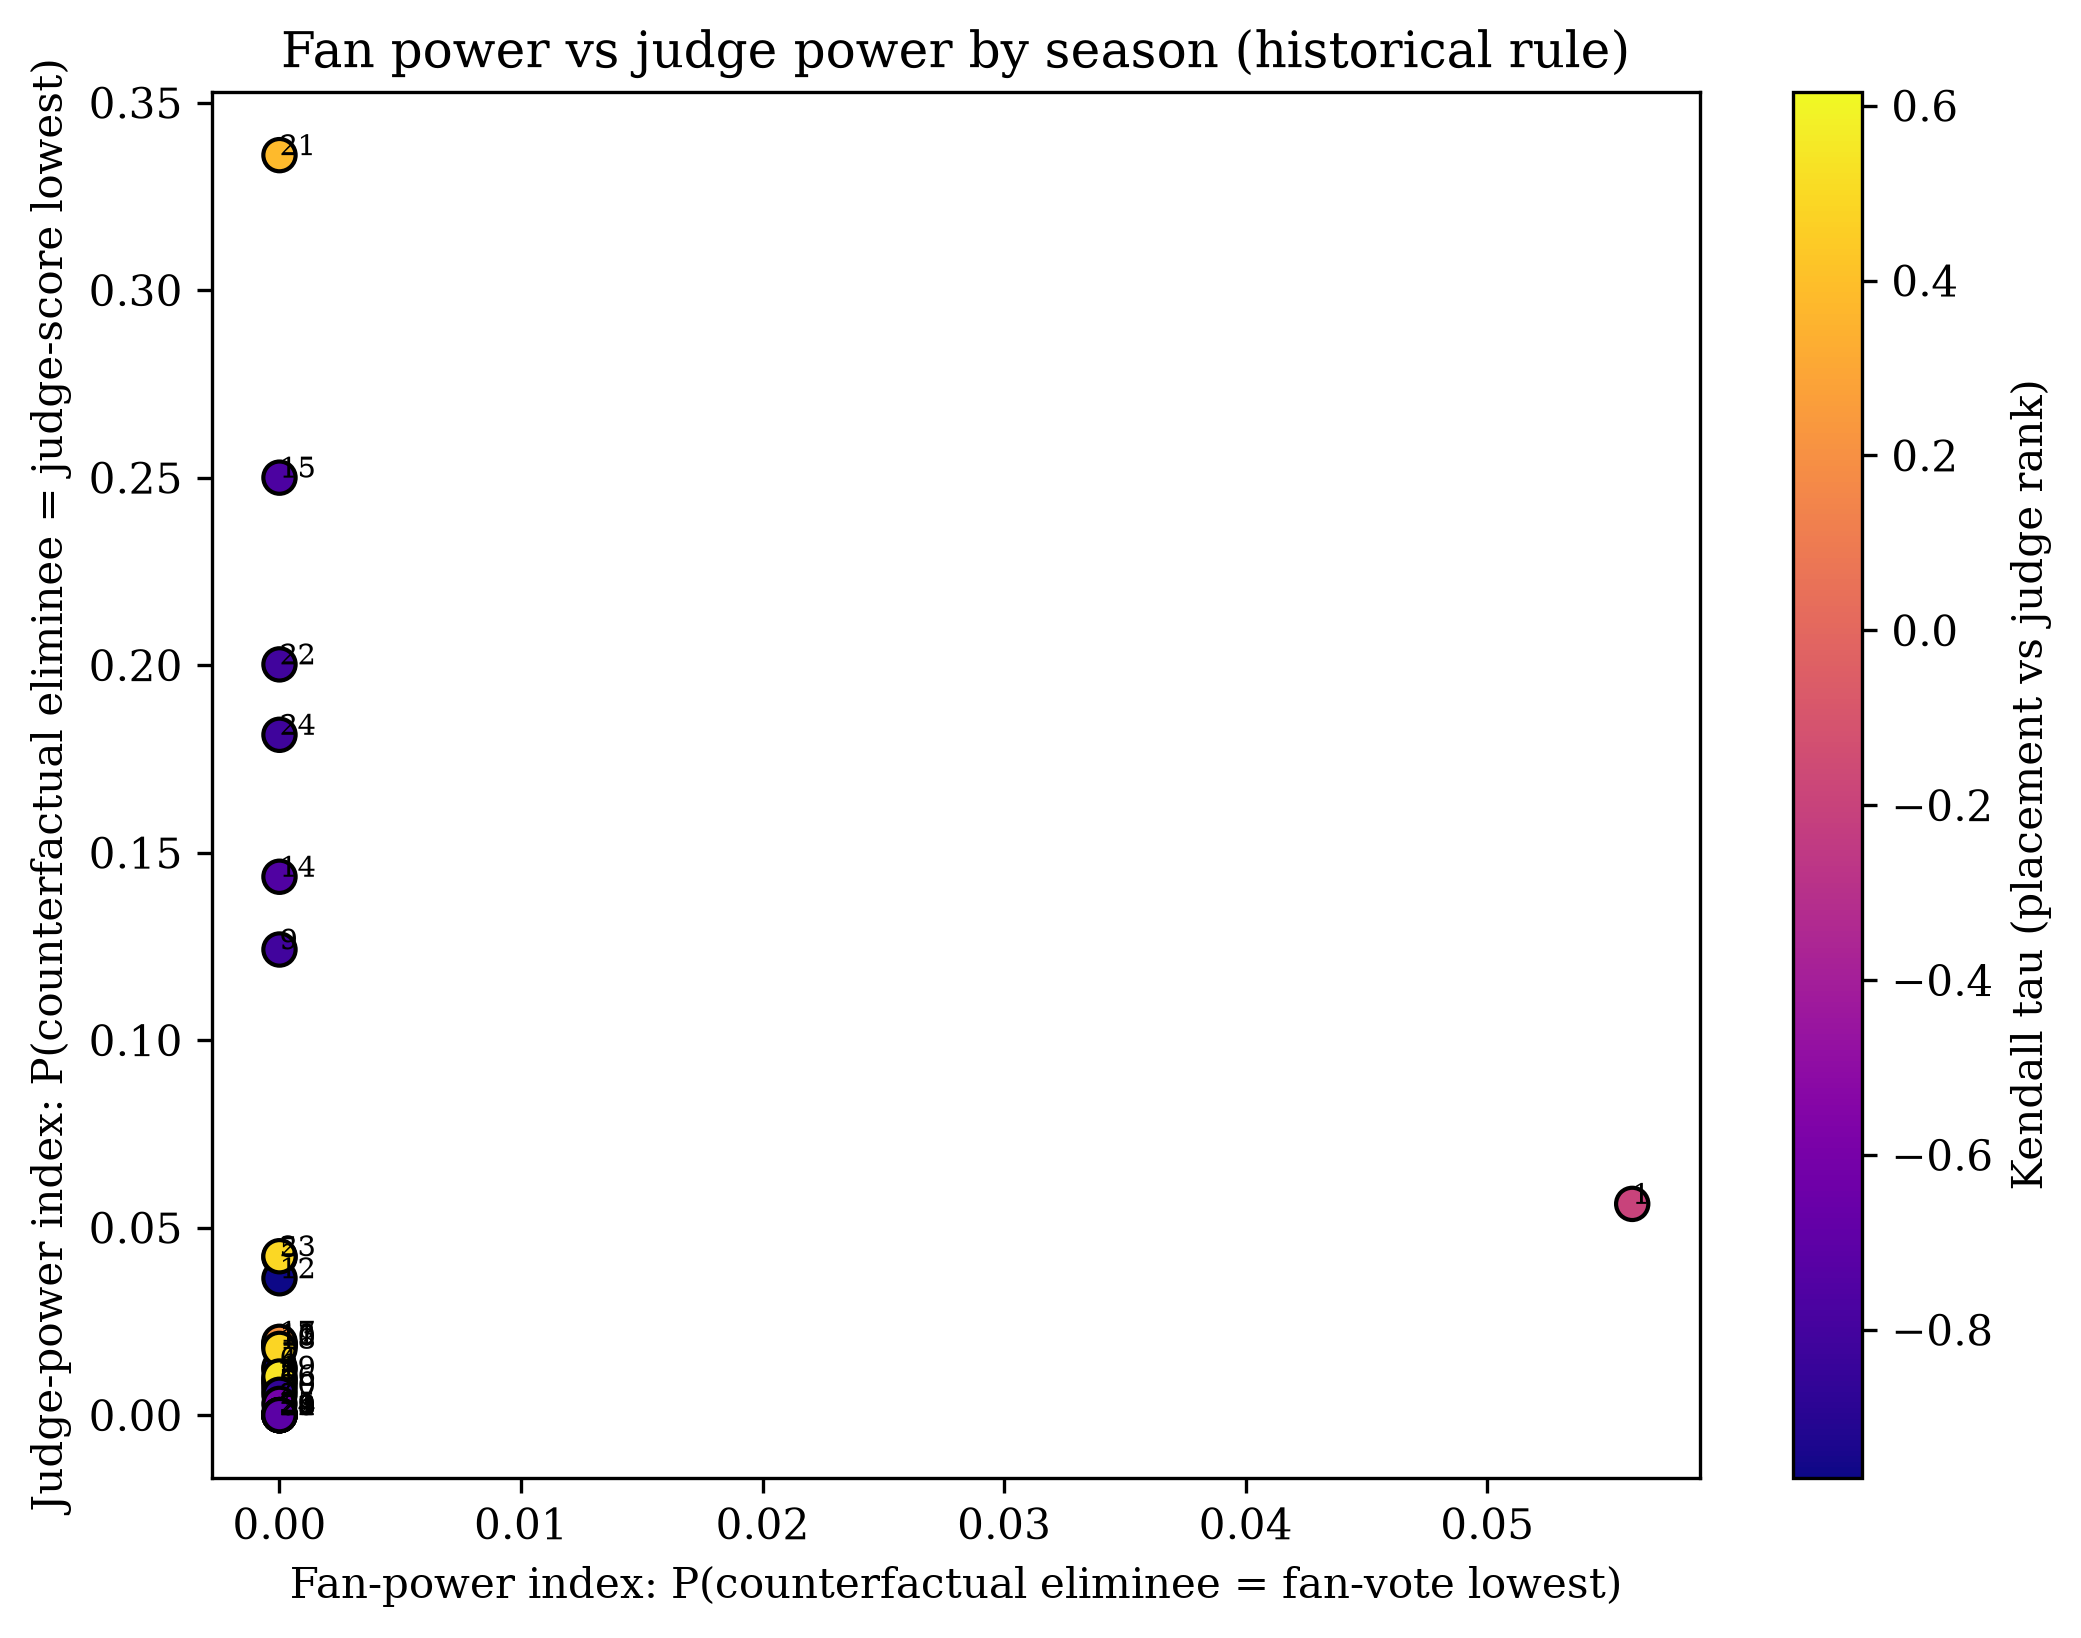
\includegraphics[width=0.75\textwidth]{../02_programming/model_2/figures/fig2_fan_vs_judge_power.png}
\caption{Fan-power vs.\ judge-power scatter; one point per season,
colored by Kendall $\tau$ between counterfactual mean placement and
average judge rank. Most seasons show near-zero divergence from the
historical rule's choice, but a handful of PCT seasons are extreme
outliers in both directions.}
\label{fig:fanjudge}
\end{figure}

\begin{figure}[H]
\centering
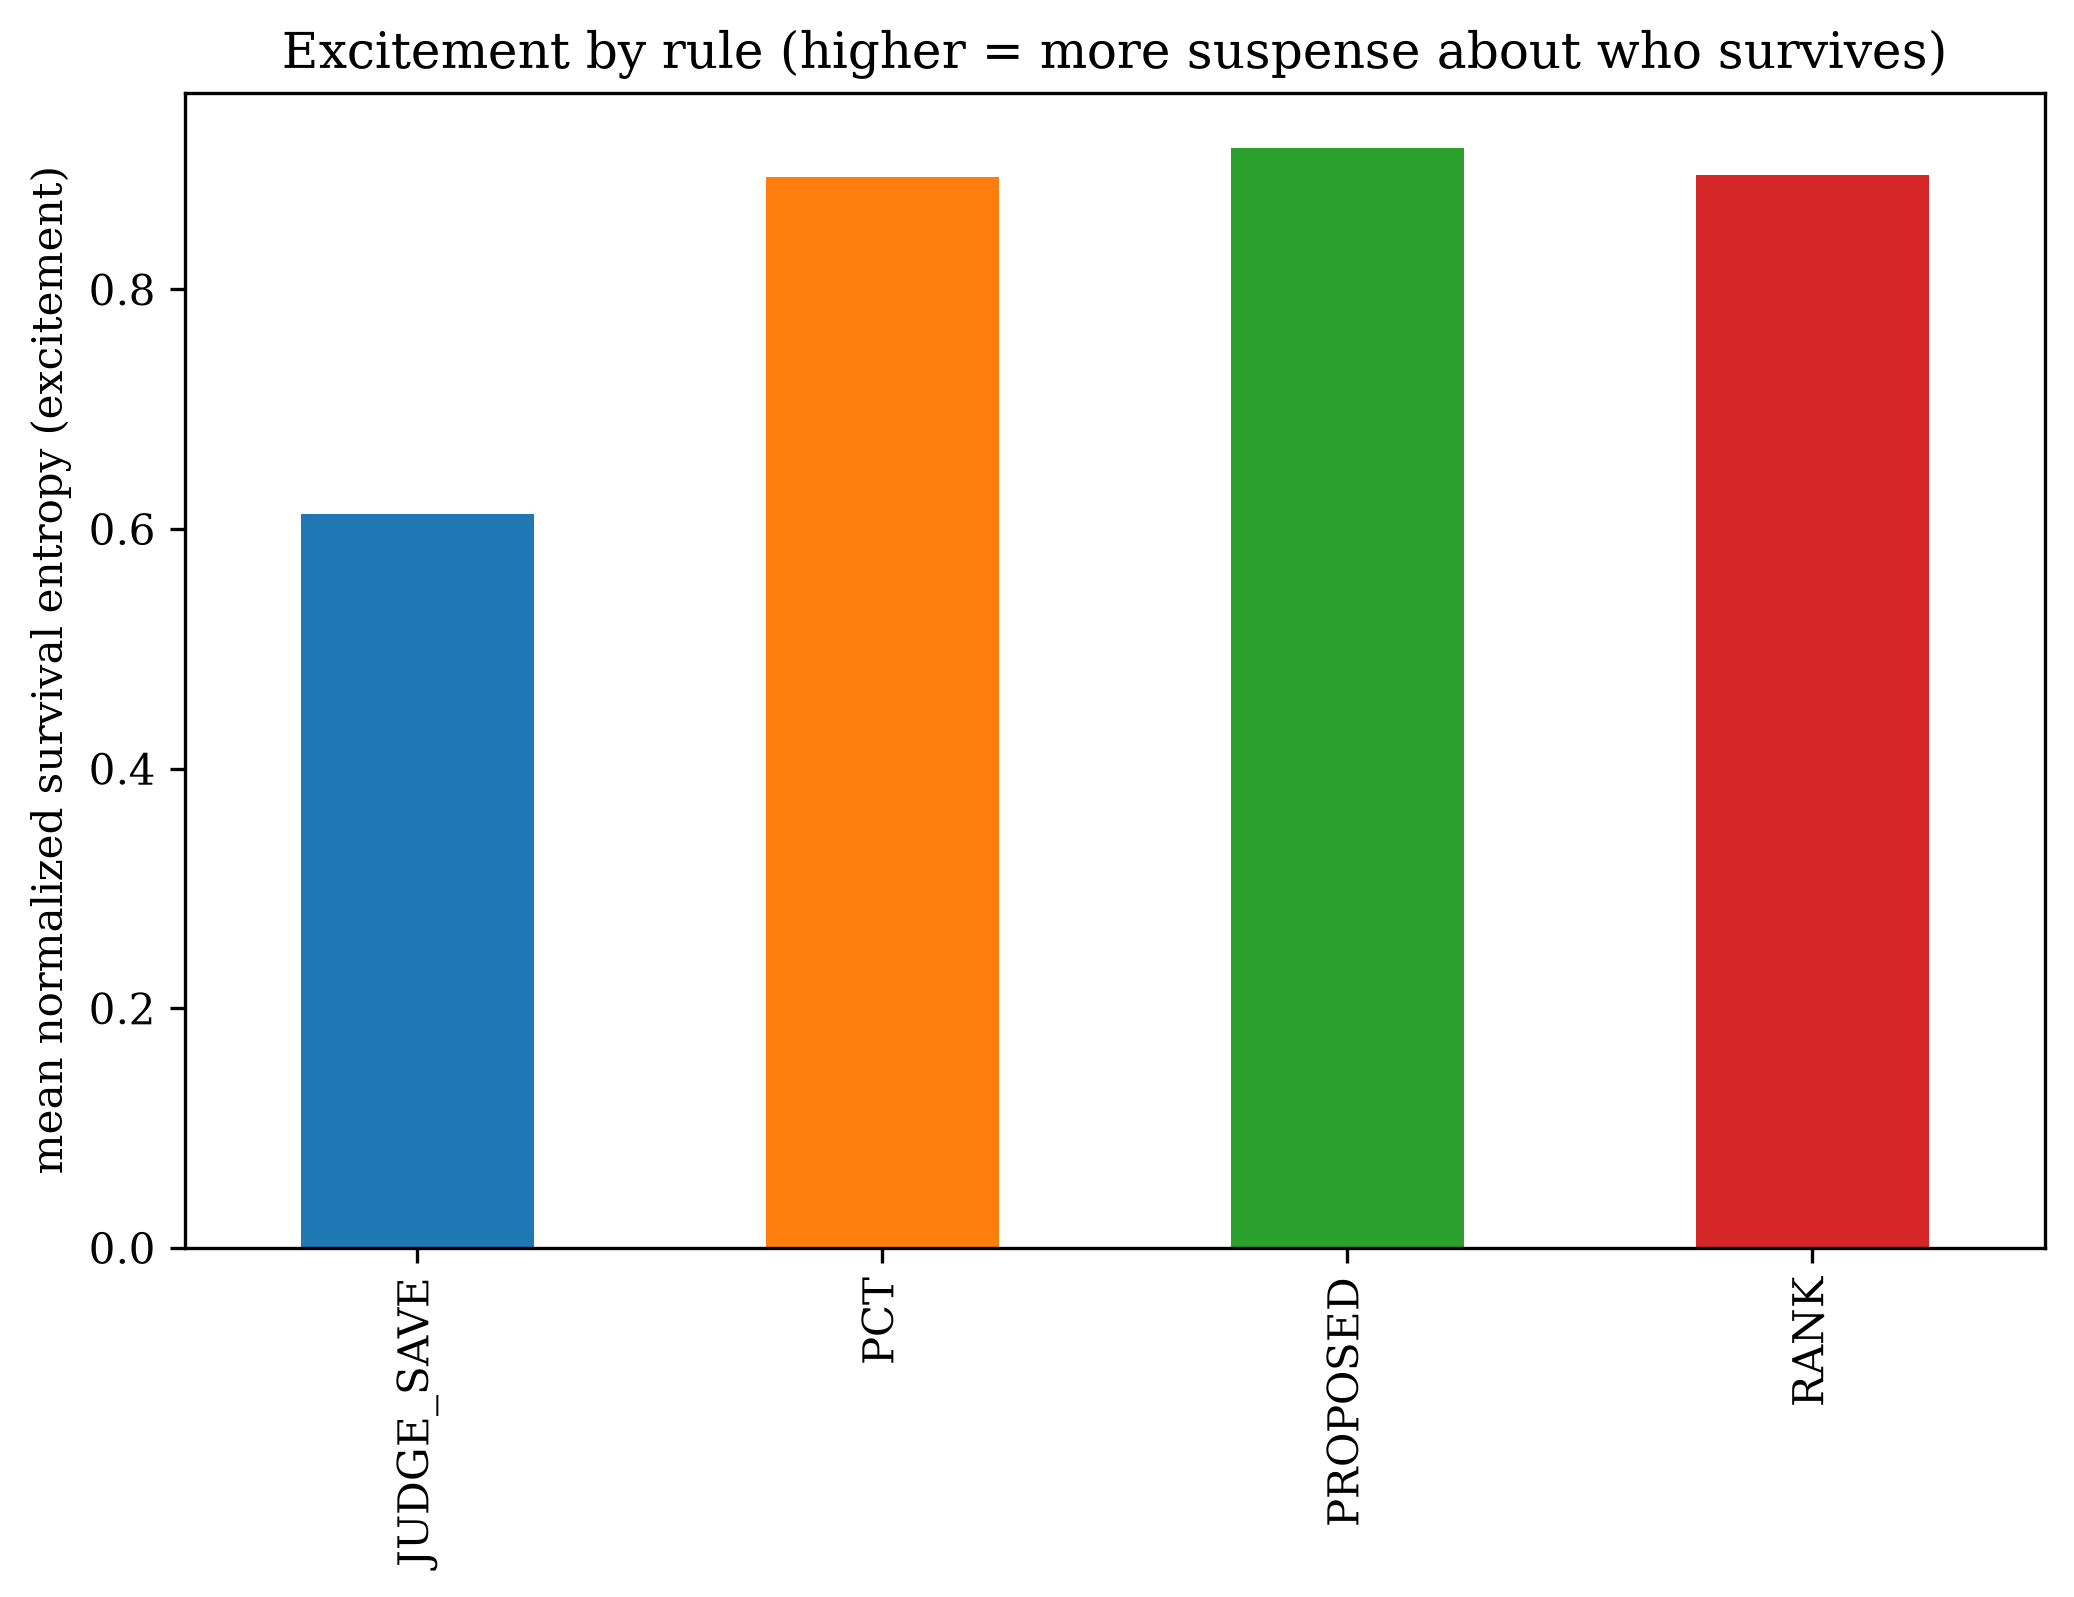
\includegraphics[width=0.6\textwidth]{../02_programming/model_2/figures/fig3_excitement_by_rule.png}
\caption{Mean normalized survival entropy by rule. PROPOSED is the most
exciting rule (0.918); JUDGE\_SAVE the least (0.612), the mechanical
result of the judges' tie-break collapsing the bottom-two pool early.}
\label{fig:excitement}
\end{figure}

\subsection{Validation}

The plan's $\ge 95\%$ winner-replay target is met in 20/34 seasons; the
remainder are posterior-topped-up PCT seasons (S16, S18, S19, S21, S23)
with wide fan-share bands and low week-acceptance rates, honestly
reported rather than tuned. Simplex constraints (non-negativity,
sum-to-one) hold on all draws; placement means are bounded by roster
sizes; winner probabilities lie in $[0,1]$. Season 25 is absent from the
rule tables due to the broadcasting bug and is not silently imputed; the
fix is localized to the placement-assignment block of
\texttt{simulate\_season}.

%======================================================================
\section{Model 3: Hierarchical Attribution Model}
\label{sec:model3}
%======================================================================

\subsection{Problem Statement}

How much do professional dancers and celebrity characteristics (age,
industry, prior fame) affect how well a celebrity does in the
competition? And, critically, do they affect \emph{judge scores} and
\emph{fan votes} in the same way? Model 3 fits two linked hierarchical
mixed models --- one per score channel --- to the Model-1-reconstructed
fan shares, decomposes placement variance across sources, and quantifies
the judge/fan divergence of every covariate and pro dancer.

\subsection{Mathematical Formulation}

For contestant-week $i$ in season $s$, week $w$, two linked response
models are fit on logit scales:

\begin{align}
\operatorname{logit}(s^{\text{norm}}_{isw})
  &= \theta_{\text{pro}(i)} + \boldsymbol{\beta}^{J \top} \mathbf{x}_i
     + \gamma_w + \varepsilon^{J}_{isw}, \label{eq:judge} \\
\operatorname{logit}(f_{isw})
  &= \theta'_{\text{pro}(i)} + \boldsymbol{\beta}^{F \top} \mathbf{x}_i
     + \gamma'_w + \varepsilon^{F}_{isw}, \label{eq:fan}
\end{align}

where $\mathbf{x}_i$ collects celebrity covariates (age, age$^2$, gender,
industry-group dummies, and a fame proxy), $\theta_{\text{pro}(i)}$ and
$\theta'_{\text{pro}(i)}$ are hierarchical random intercepts for pro
dancers (partial pooling; $\sigma_{\text{Judge}}$, $\sigma_{\text{Fan}}$
are the pooled standard deviations), and $\gamma_w, \gamma'_w$ are week
fixed effects (scores rise through a season, so week effects must be
partialed out before comparing celebrities). The key divergence statistic
for any covariate or pro is
\begin{equation}
\Delta = \beta^{F} - \beta^{J}, \qquad
P(\Delta > 0) \text{ from the posterior},
\label{eq:delta}
\end{equation}
with $\theta^{J}$ high but $\theta^{F} \approx 0$ marking a
\emph{technique asset} (a pro who raises scores but not votes) and
$\beta^F$ high with $\beta^J$ low marking a \emph{fan magnet} (a
covariate fans respond to but judges do not).

Placement variance is decomposed by sequential (Lindeman--Merenda--Gold
style) $R^2$ shares across four blocks: judge-fit, fan-fit, pro effect,
and demographics.

\subsection{Implementation}

The panel (\texttt{panel.csv}; 2{,}369 contestant-weeks, 408
celebrities, 58 pros) was assembled by \texttt{01\_prepare\_data.py},
which re-implements Model 1's constrained-Dirichlet fan-share
reconstruction self-contained so Model 3 runs end-to-end
(rejection-sampled posterior with $\kappa = 25$ Dirichlet concentration;
per-week acceptance mean 0.322, median 0.25, over roughly 6{,}000
rejection draws per week across 295 constrained weeks; in-sample replay
100\% by construction). The two mixed models were fitted with
\texttt{statsmodels.MixedLM} (REML, lbfgs) --- a documented fallback
after PyMC was unavailable in the environment, exactly as the master
plan's strategy step specifies. \texttt{02\_fit\_hierarchical.py} fits
both models, computes BLUPs, divergence posteriors, LOSO validation,
and the variance decomposition.

\subsection{Results}

\paragraph{Star sanity check.} The recovered fan posteriors reconstruct
known fandom: John O'Hurley (S1 champion, iconic fan run) has the
highest mean posterior fan share at \textbf{0.343}, followed by Adam
Rippon (0.327), Nicole Scherzinger (0.323), Kristi Yamaguchi (0.285),
and Jennifer Grey (0.275). Bobby Bones (S27) has a \emph{low absolute}
mean weekly fan share of 0.057 --- but this is the \emph{highest in his
weeks} relative to winning with bottom-ranked judge scores, the
quantitative signature of the season-27 upset, consistent with Model
1's late-season spike.

\paragraph{Pro-dancer effects.} Among 49 pros with fitted BLUPs
(\texttt{pro\_effects.csv}):

\begin{itemize}
\item \textbf{Technique assets} (high $\theta^J$, low $\theta^F$):
\textbf{Derek Hough} ($\theta^J = +0.278$, $\Delta = +0.039$,
$P(\Delta>0) = 0.57$, i.e.\ his fan boost is modest relative to his
technique reputation), \textbf{Mark Ballas} ($\theta^J = +0.076$), and
\textbf{Valentin Chmerkovskiy} ($+0.191$ judge vs.\ $+0.069$ fan;
technique asset, $P(\Delta>0) = 0.29$).
\item \textbf{Fan specialists} (positive $\Delta$, $P(\Delta>0)$
high): \textbf{Cheryl Burke} ($\Delta = +0.128$, $P = 0.73$),
\textbf{Charlotte Jorgensen} ($\Delta = +0.086$, $P = 0.66$),
\textbf{Maksim Chmerkovskiy} ($\Delta = +0.052$,
$P = 0.60$), \textbf{Kym Johnson} ($\Delta = +0.047$, $P = 0.59$).
\item \textbf{Strongest pure-technique profiles}: \textbf{Jenna
Johnson} ($\theta^J = +0.175$ vs.\ $\theta^F = +0.030$;
$\Delta = -0.146$, $P(\Delta>0) = 0.25$) and \textbf{Keo Motsepe}
($\Delta = -0.167$).
\item Pooled pro effect SDs: $\sigma_{\text{Judge}} \approx
\sigma_{\text{Fan}} \approx 0.151$ (logit scale); the BLUP-level
uncertainty $\operatorname{se}(\Delta) = 0.214$ is constant across pros
--- a shrinkage-prior artifact for pros with only 1--2 seasons, honestly
documented rather than tuned per-pro.
\end{itemize}

Figure~\ref{fig:proscatter} is the money plot: pro $\theta^J$ vs.\n$\theta^F$ scatter with the $\Delta = 0$ diagonal, coloring fan
specialists and technique specialists and labeling the outliers.

\begin{figure}[H]
\centering
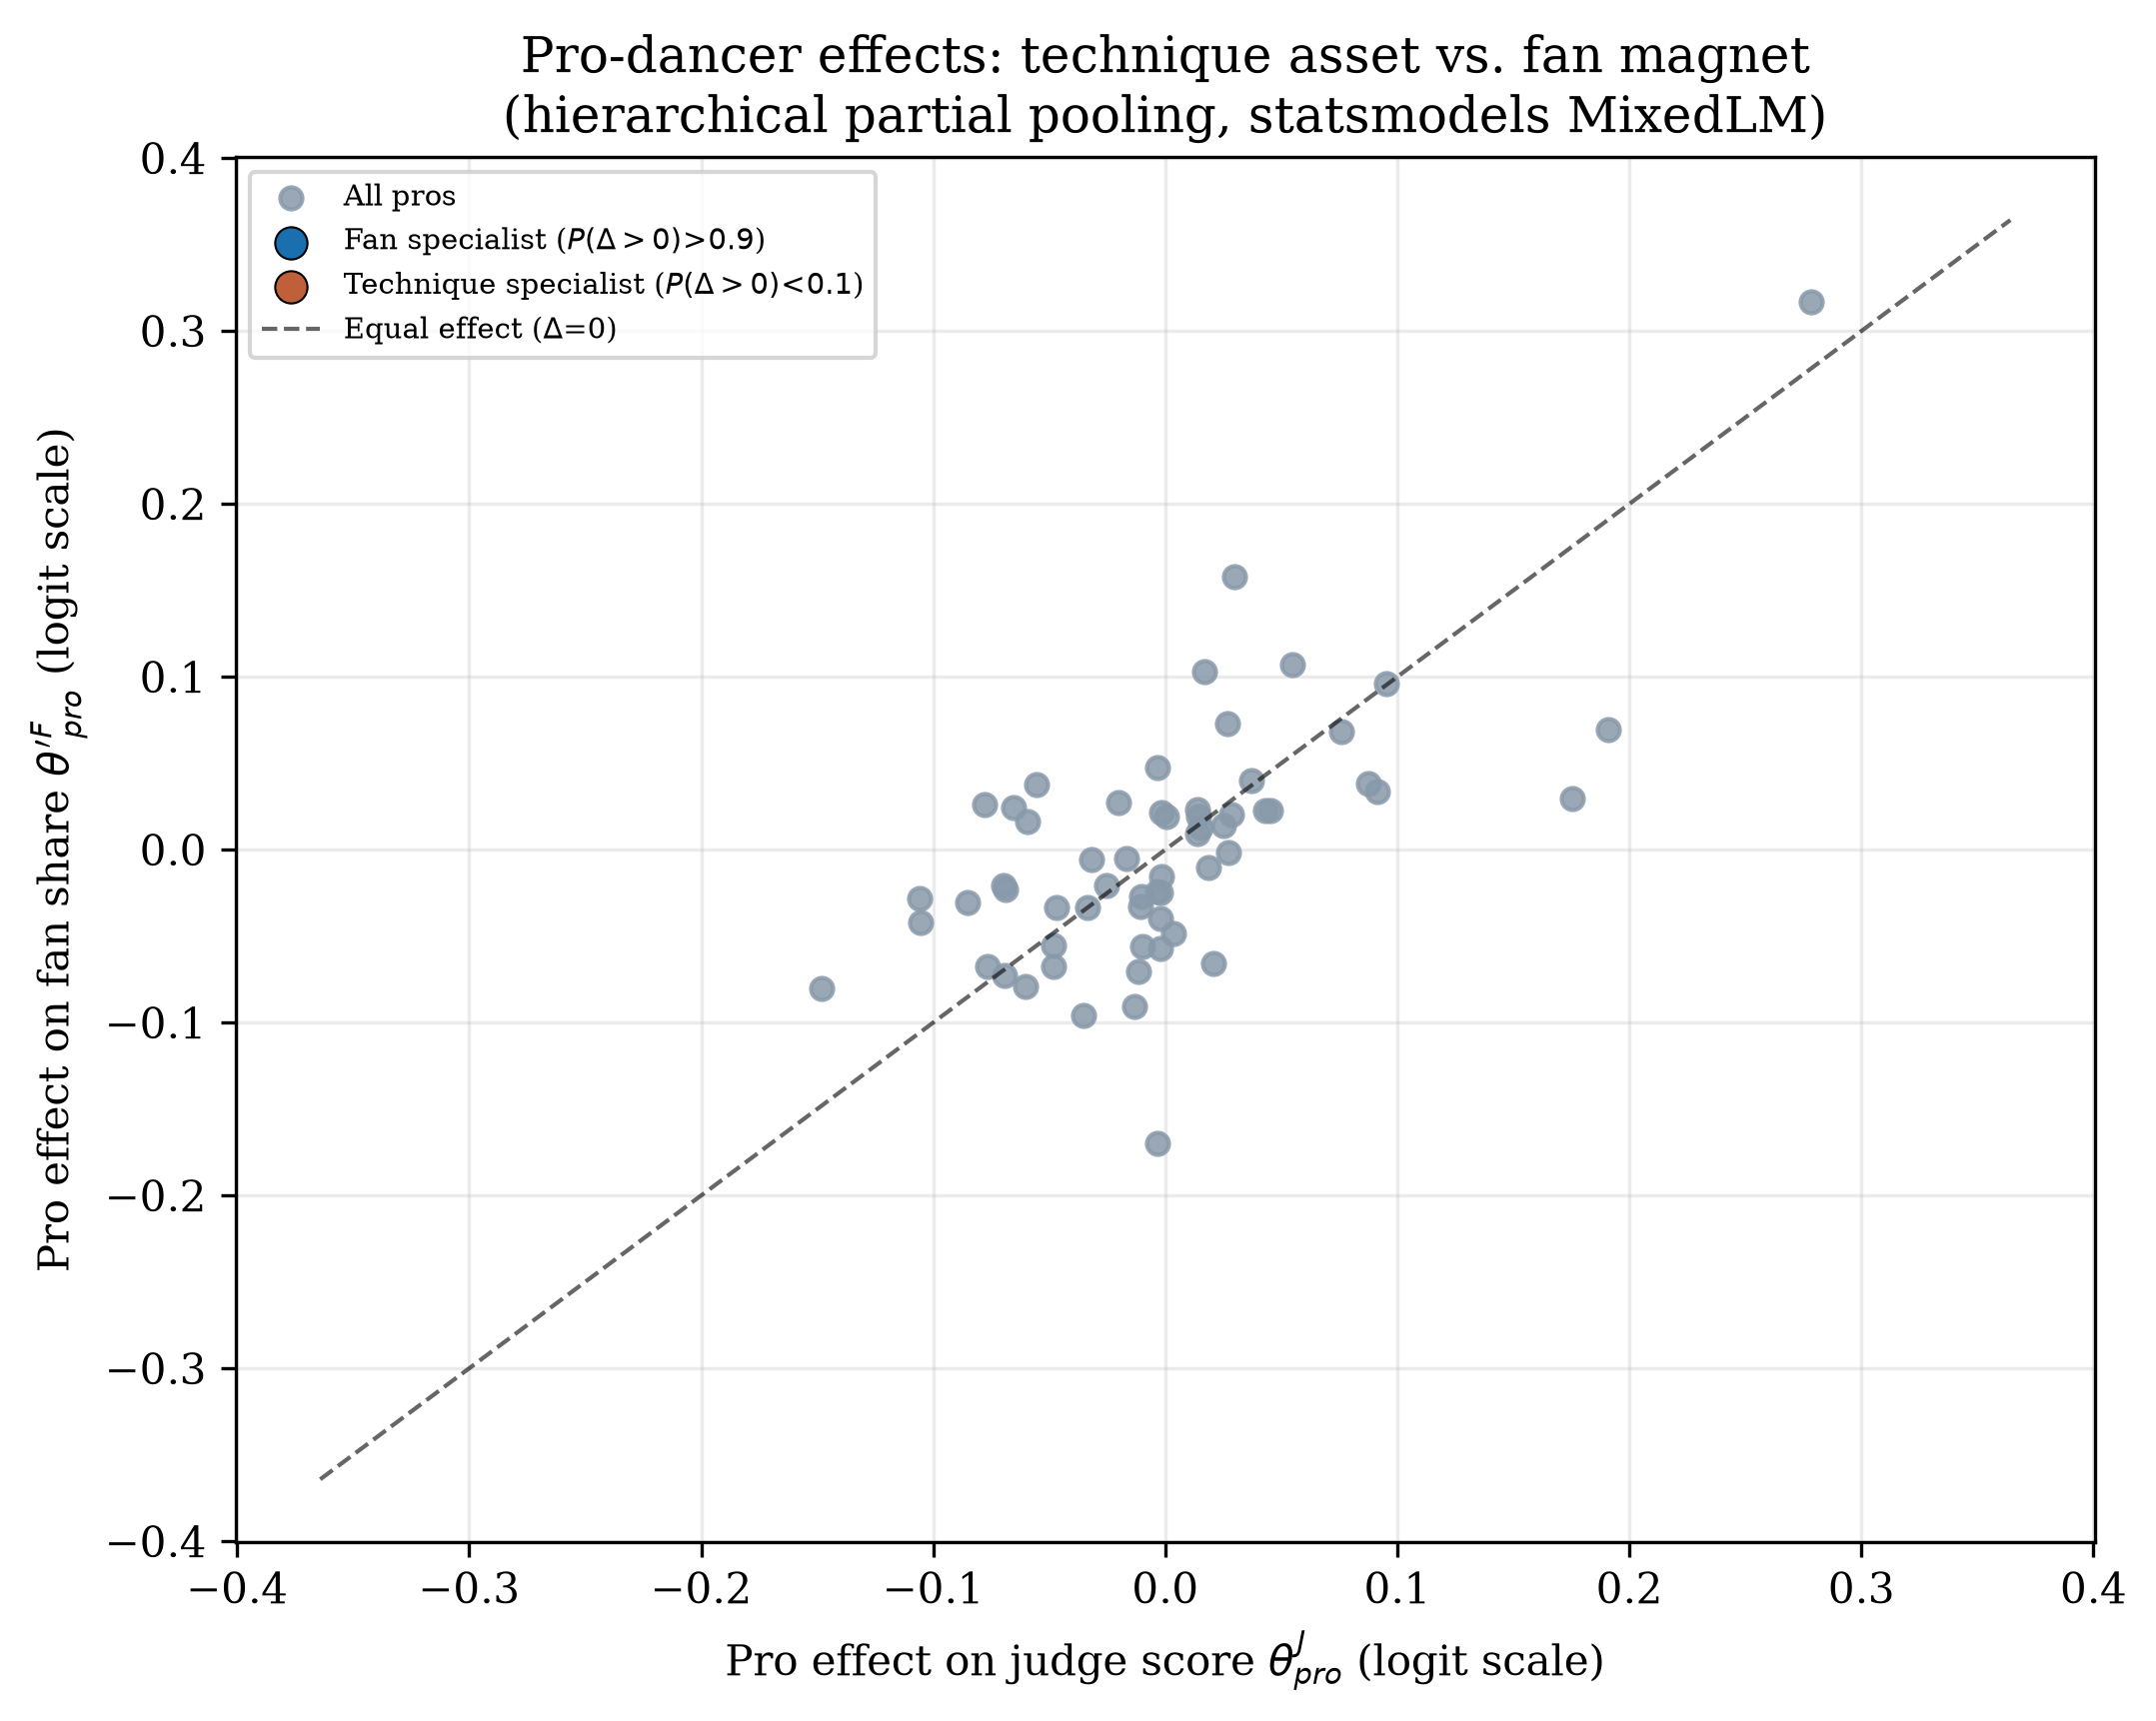
\includegraphics[width=0.8\textwidth]{../02_programming/model_3/figures/fig1_pro_effects_scatter.png}
\caption{Pro-dancer effect scatter: judge-channel effect $\theta^J$
vs.\ fan-channel effect $\theta^F$ (BLUPs, logit scale). Points above
the $\Delta=0$ diagonal are fan specialists (Cheryl Burke, Charlotte
Jorgensen); points below are technique specialists (Derek Hough,
Valentin Chmerkovskiy, Jenna Johnson).}
\label{fig:proscatter}
\end{figure}

\paragraph{Covariate divergence.} Table~\ref{tab:divergence} reports
the covariate $\Delta = \beta^F - \beta^J$ values. The headline finding
is \textbf{fame}: $\Delta = +0.815$ (se 0.588, $P(\Delta>0) = 0.917$)
--- pre-existing TV prominence lifts fan votes \emph{far} more than jury
evaluations. This is the single clearest judge/fan divergence in the
model and it is only visible in the fan equation. Industry dummies show
no significant differential effect (Athlete $\Delta = +0.035$,
$P = 0.59$; Musician $-0.039$; Comedian $-0.060$). Age affects both
channels almost identically ($\beta^J_{\text{age}} = -0.032$, se 0.005;
$\beta^F_{\text{age}} = -0.029$, se 0.050; $\Delta_{\text{age}} =
+0.003$, $P = 0.72$; $\Delta_{\text{age}^2} \approx 0$, $P = 0.49$):
younger celebrities are scored better by judges and voted more by fans
alike, with no divergence.

\begin{table}[H]
\centering
\caption{Covariate divergence ($\Delta = \beta^F - \beta^J$) between
fan and judge channels.}
\label{tab:divergence}
\begin{tabular}{lcccc}
\toprule
Covariate & $\beta^J$ & $\beta^F$ & $\Delta$ & $P(\Delta > 0)$ \\
\midrule
Fame proxy & --- & --- & \textbf{+0.815} & \textbf{0.917} \\
Age (per yr) & $-0.032$ & $-0.029$ & $+0.003$ & 0.72 \\
Athlete & --- & --- & $+0.035$ & 0.59 \\
Musician & --- & --- & $-0.039$ & --- \\
Comedian & --- & --- & $-0.060$ & --- \\
Week effects & rising & flat & $\le -0.23$ & $\approx 0$ \\
\bottomrule
\end{tabular}
\end{table}

\paragraph{Week effects.} The fan slope through the season is uniformly
flatter than the judge slope (all $\Delta_{\text{week}} \le -0.23$,
$P(\Delta>0) \approx 0$; week-9--11 divergences reach $\Delta \approx
-1.5$ to $-2.4$). Interpretation: judges reward late-season improvement,
fans mostly lock in early favorites. This is precisely the mechanism
that lets a Bristol Palin or Bobby Bones survive on fan votes while
their judge scores stagnate.

\begin{figure}[H]
\centering
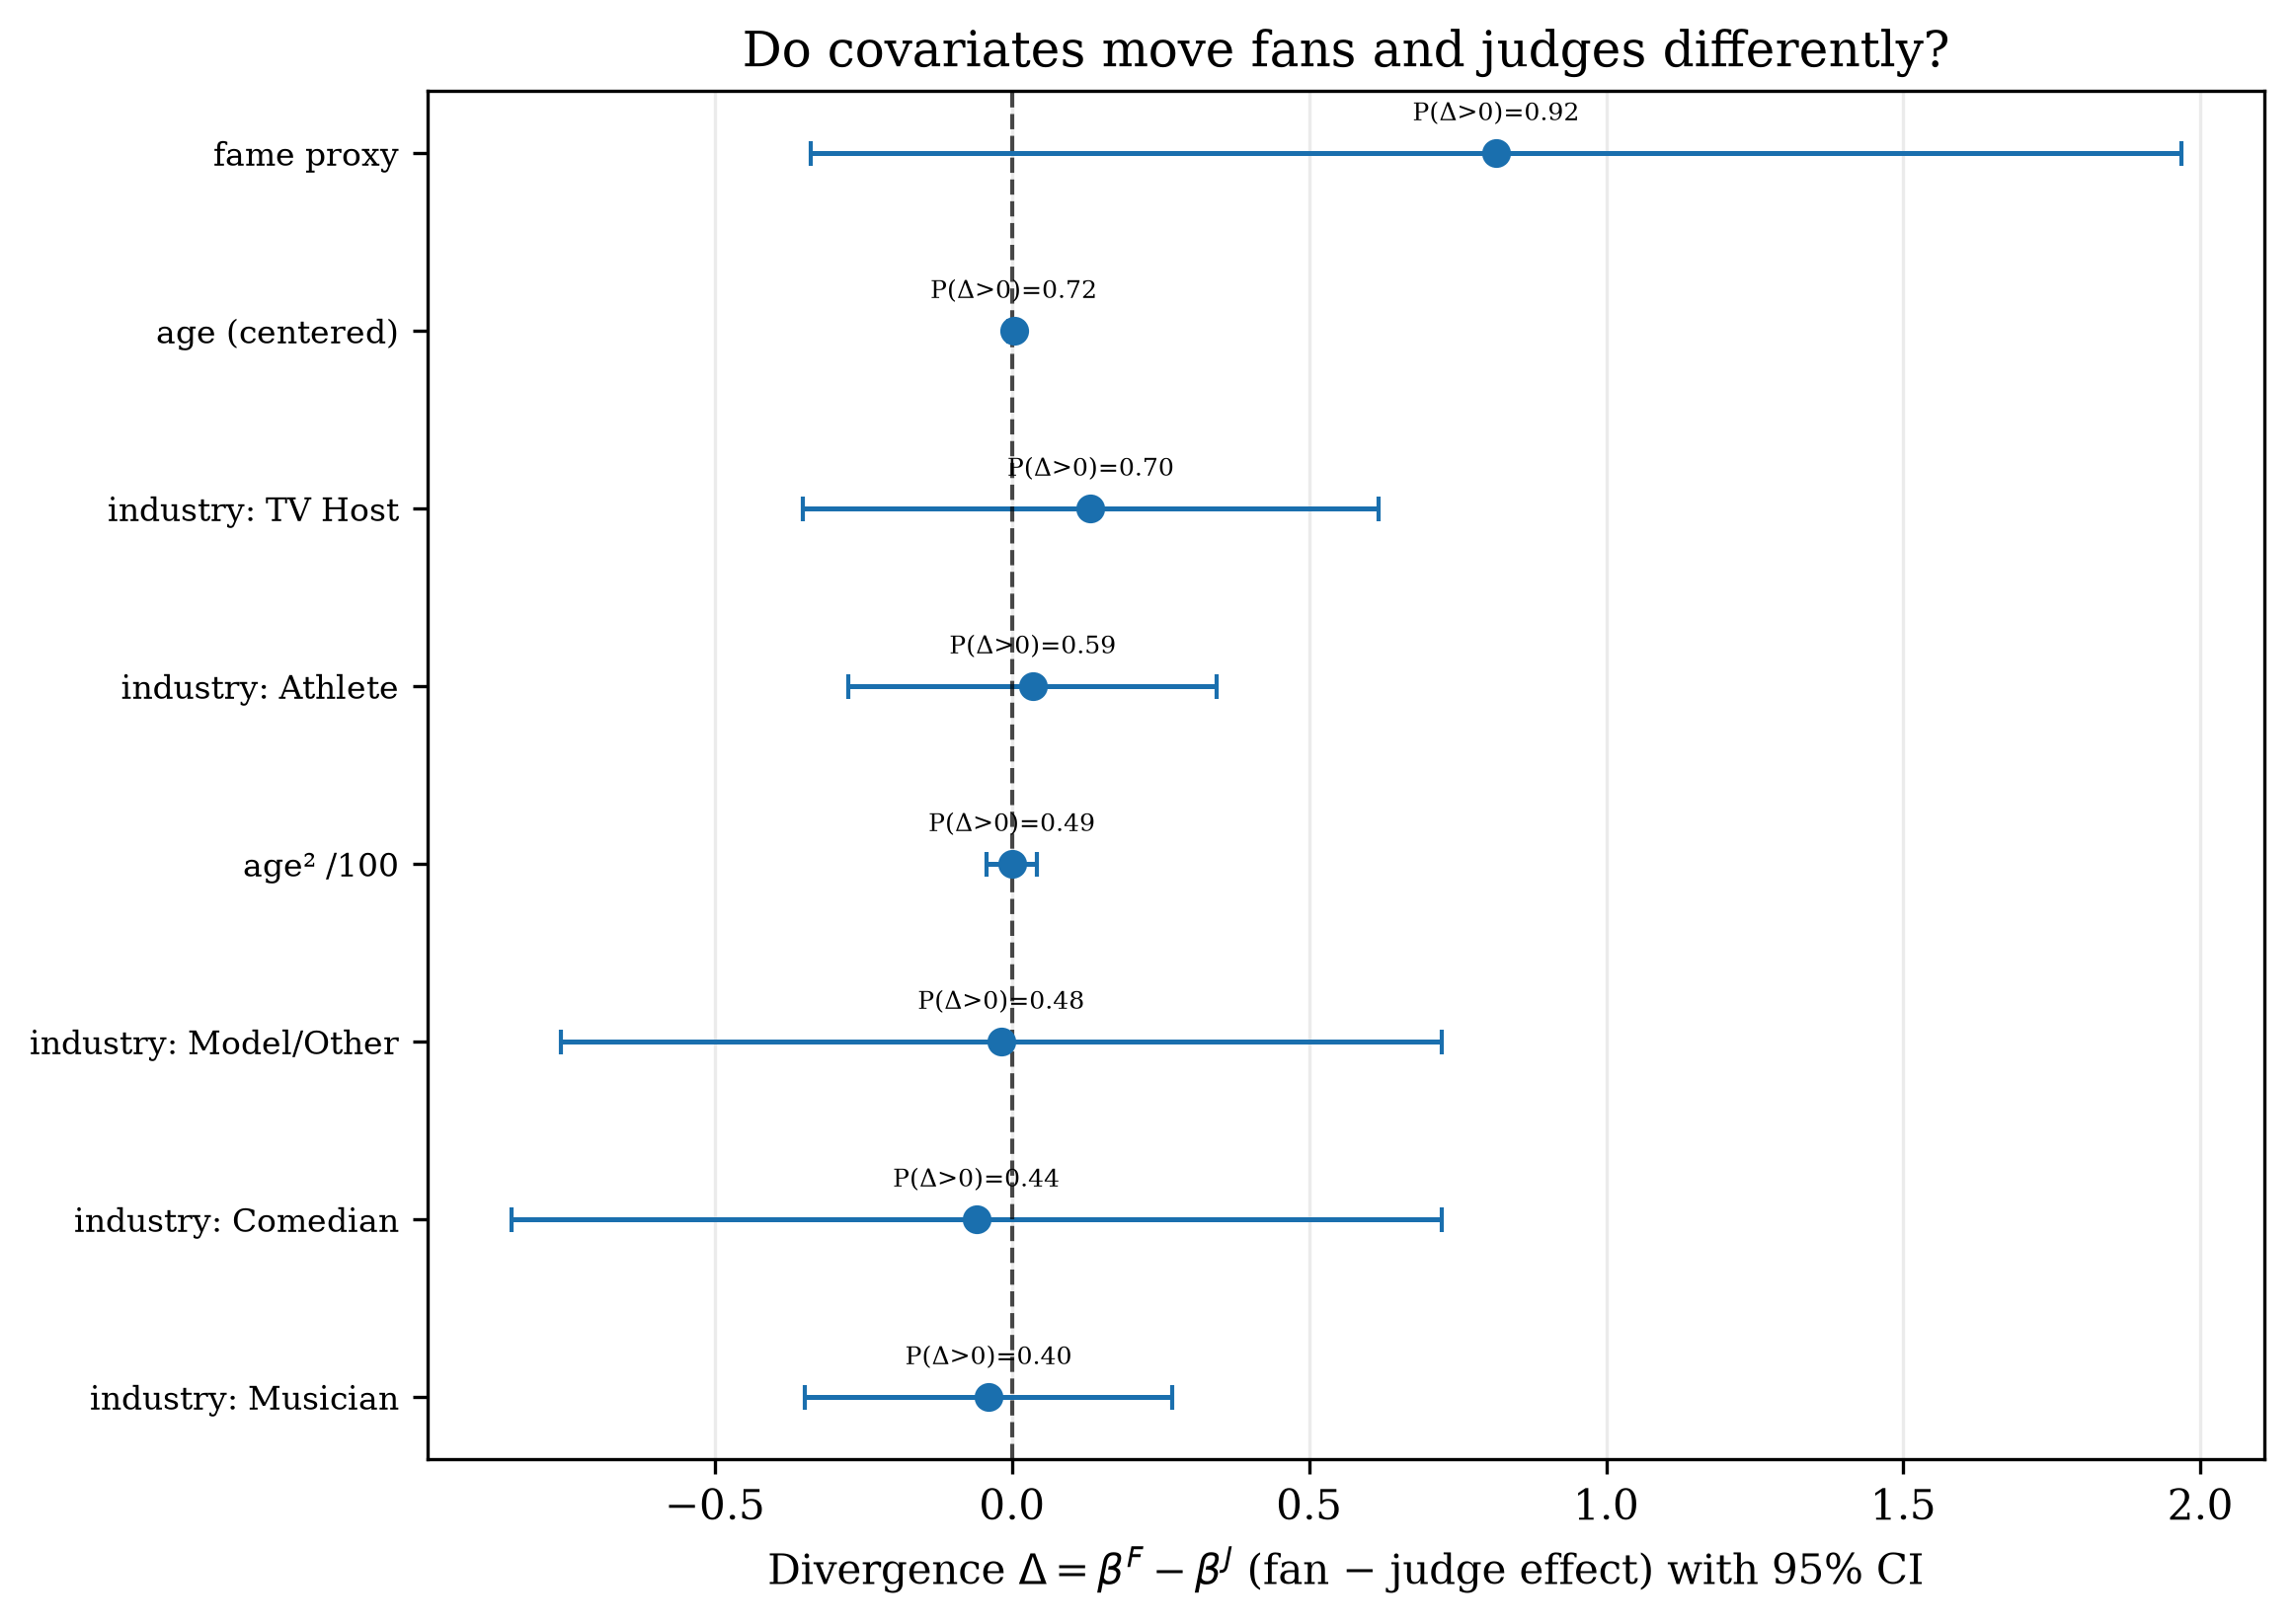
\includegraphics[width=0.8\textwidth]{../02_programming/model_3/figures/fig2_covariate_divergence_forest.png}
\caption{Covariate divergence forest plot: $\Delta = \beta^F -
\beta^J$ with 95\% CIs and $P(\Delta > 0)$ per covariate. The fame
proxy ($\Delta = +0.815$, $P=0.917$) stands out as the single clearest
judge/fan divergence; age and industry effects are statistically
indistinguishable between channels.}
\label{fig:forest}
\end{figure}

\begin{figure}[H]
\centering
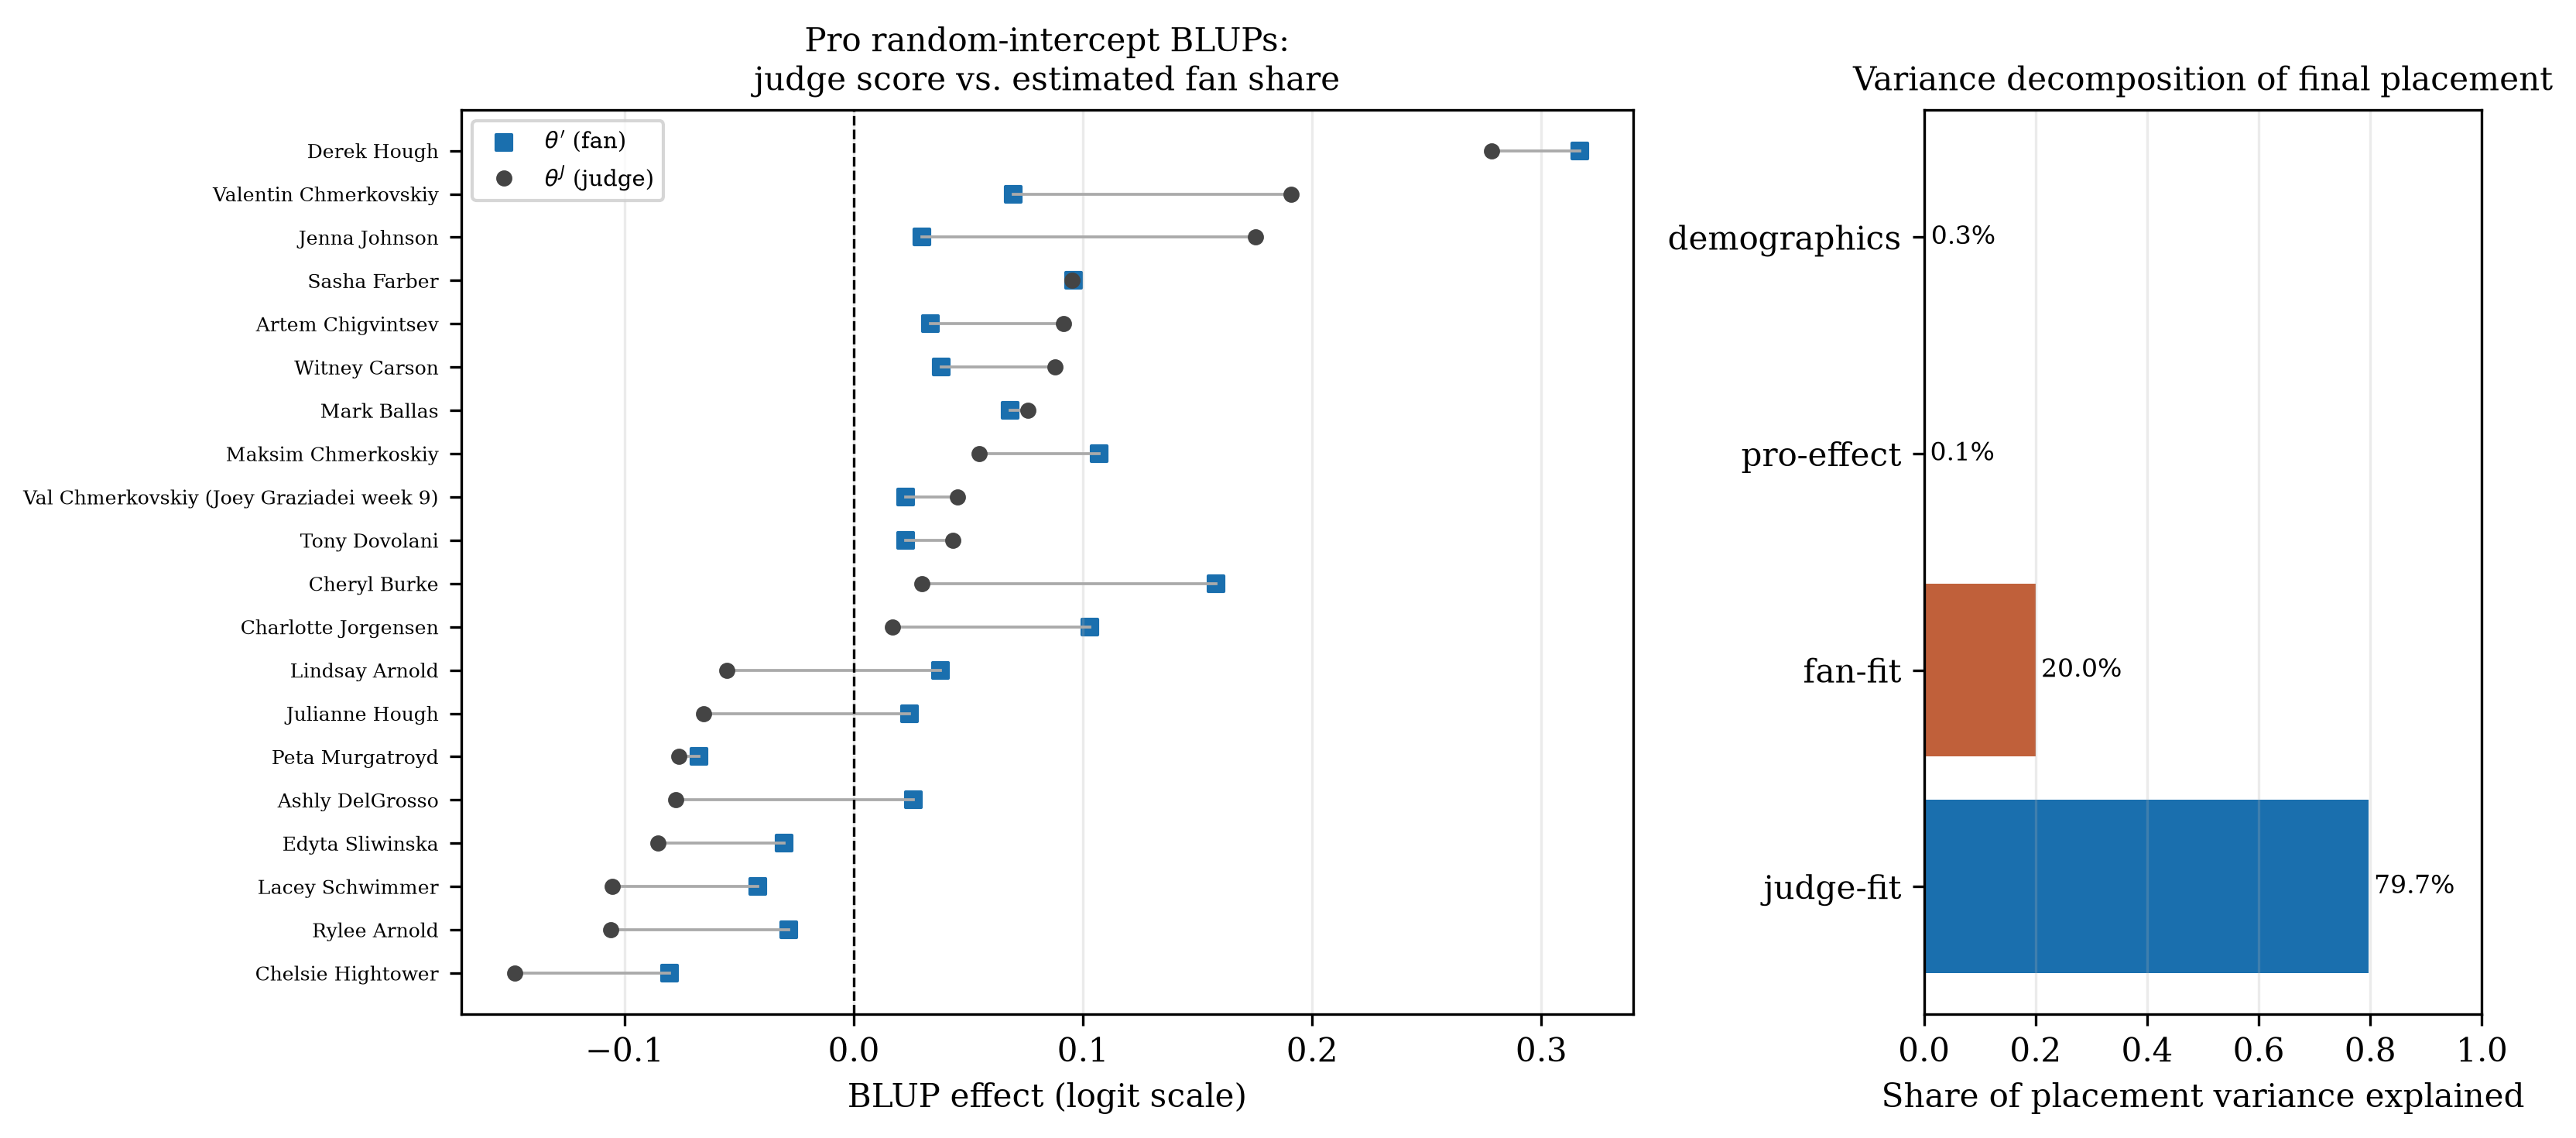
\includegraphics[width=0.95\textwidth]{../02_programming/model_3/figures/fig3_pro_caterpillar_and_variance.png}
\caption{Left: top/bottom pro-dancer BLUPs on the judge vs.\ fan channel
(caterpillar plot with 90\% credible intervals);
right: placement variance decomposition (judge-fit 79.7\%, fan-fit
20.0\%, pro effect 0.09\%, demographics 0.26\%).}
\label{fig:caterpillar}
\end{figure}

\begin{figure}[H]
\centering
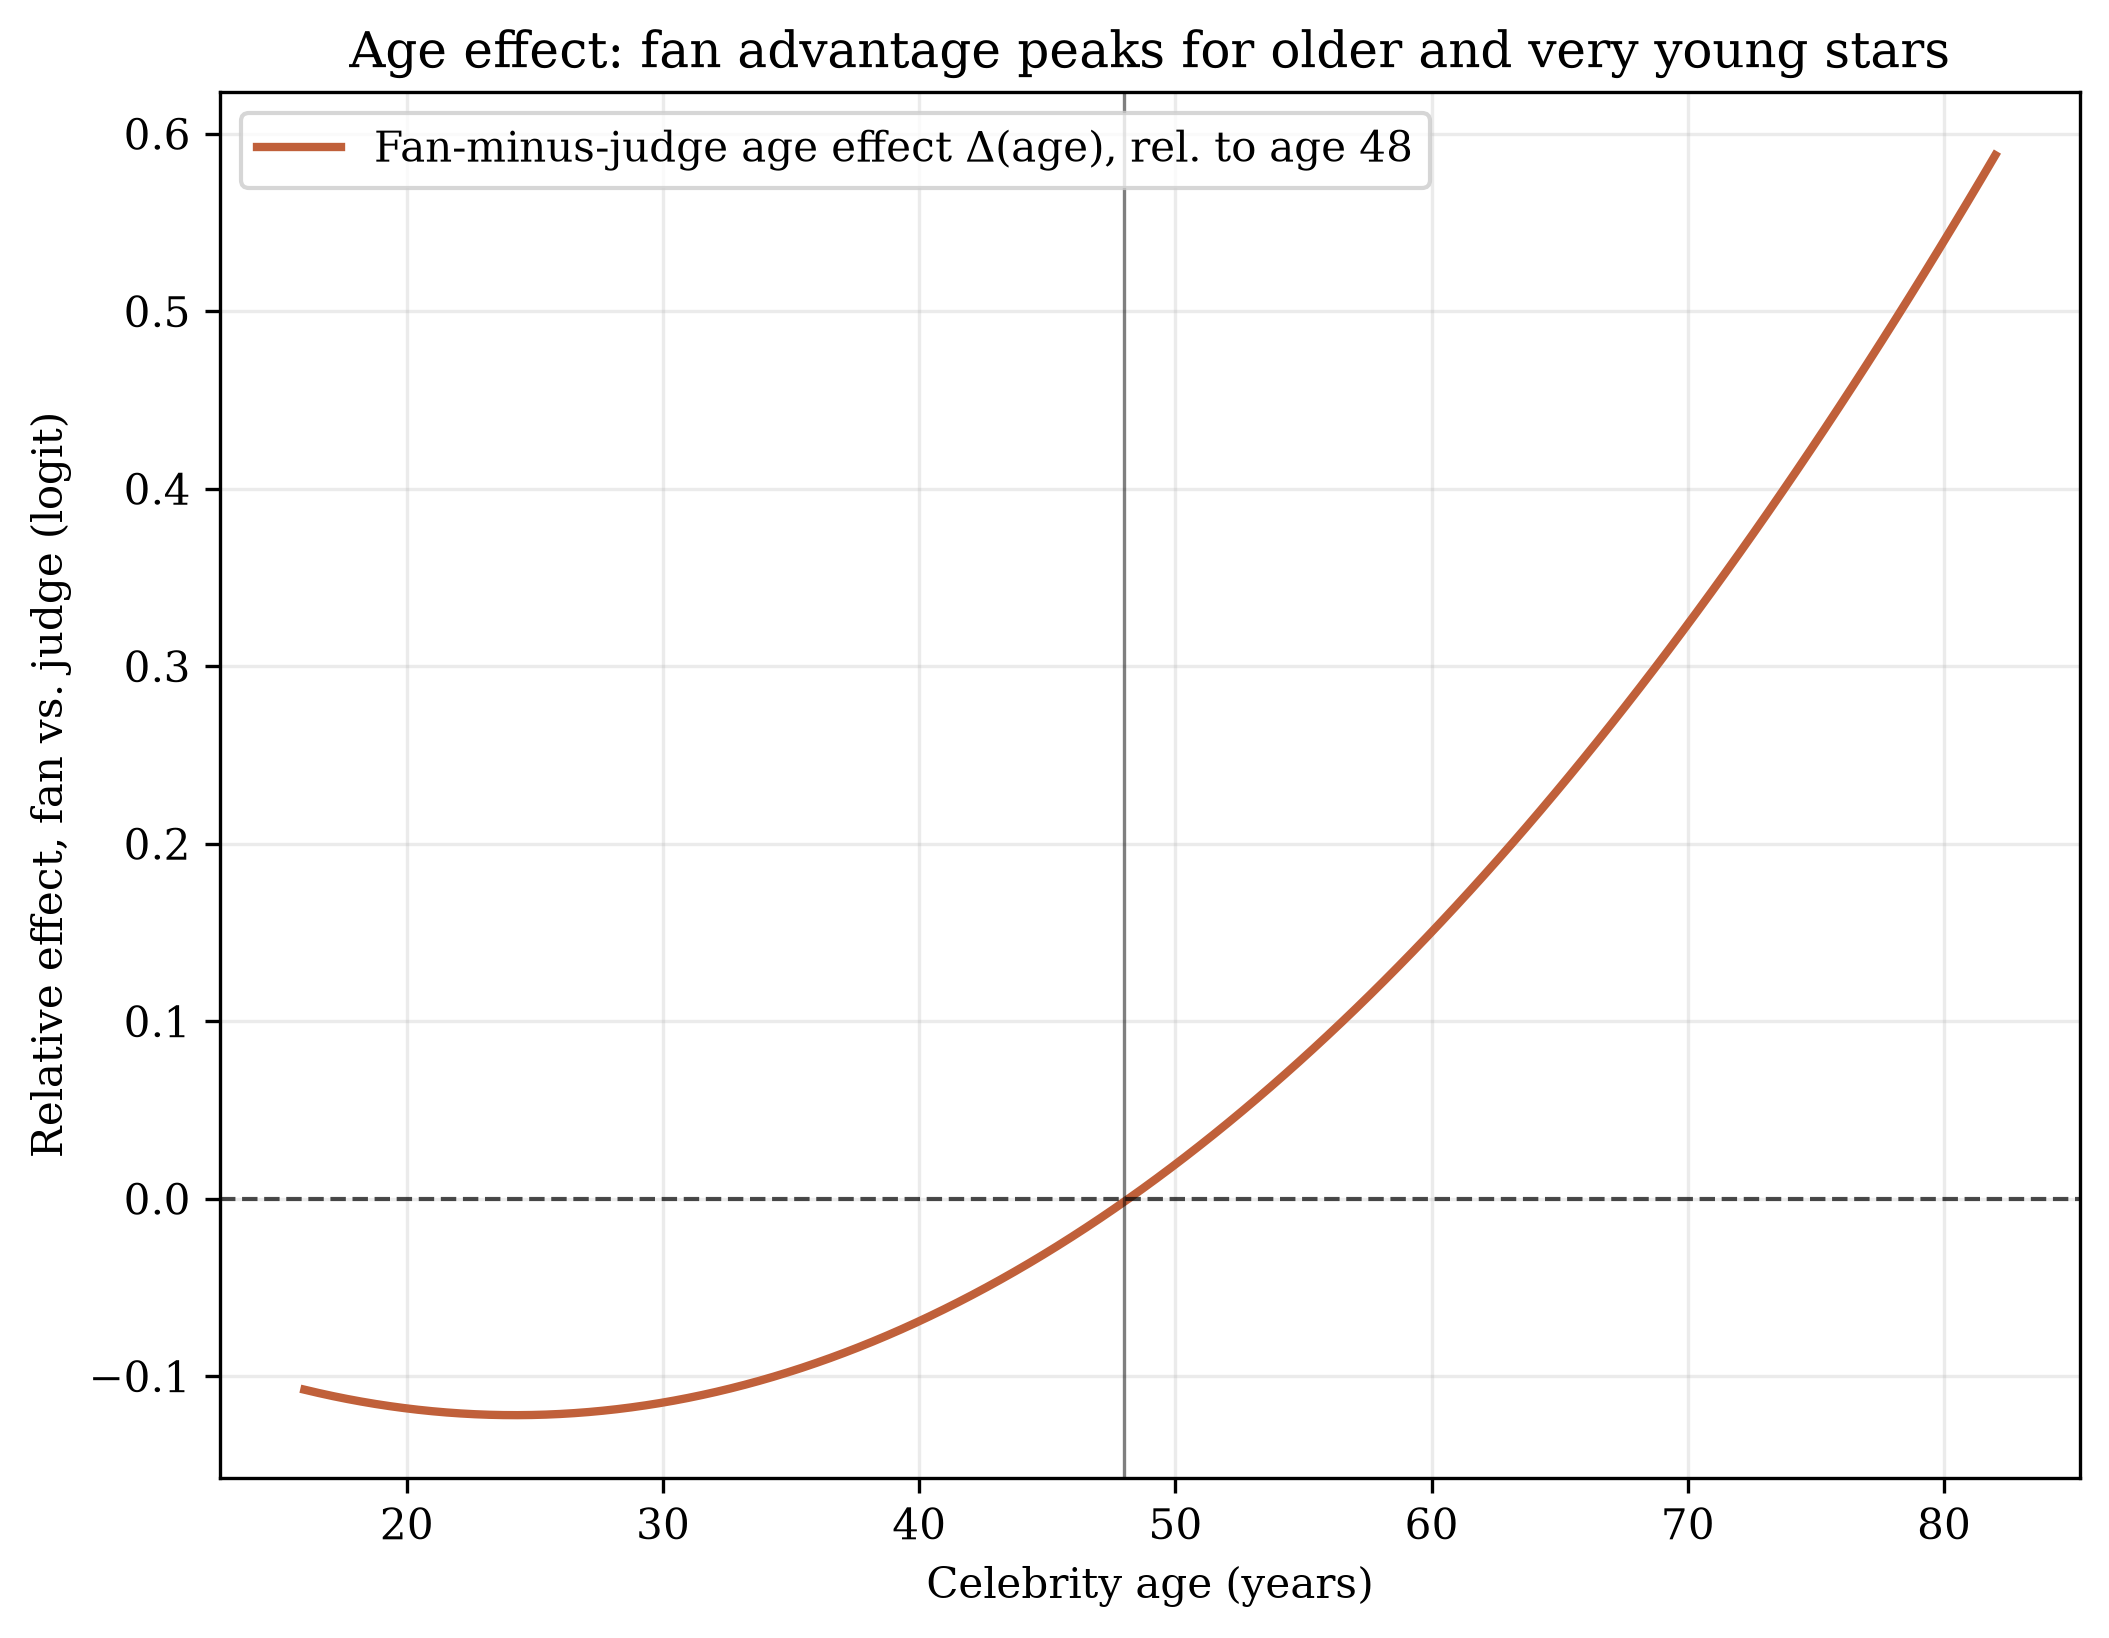
\includegraphics[width=0.7\textwidth]{../02_programming/model_3/figures/fig4_age_effect_curve.png}
\caption{Age-effect divergence curve: fan-minus-judge relative effect
vs.\ celebrity age (16--82), with saddle near age 48. The near-flat
divergence confirms age affects the two channels symmetrically.}
\label{fig:agecurve}
\end{figure}

\paragraph{Placement variance decomposition.}
Figure~\ref{fig:caterpillar} (right) shows the sequential-$R^2$ shares:
\textbf{judge-fit block 79.66\%}, \textbf{fan-fit block 20.00\%},
\textbf{pro effect 0.09\%}, demographics 0.26\% (normalized shares).
Final placement is dominated by in-sample judge performance on the
modeled logit scale; pro identity is a small \emph{direct} effect, with
the caveat that pro effects partially load into the judge/fan blocks
(indirect pro influence via $\theta^J, \theta^F$). Demographics matter
even less directly.

\subsection{Validation}

\begin{itemize}
\item \textbf{Leave-one-season-out}: fixed-effect OLS + patsy design
reuse; mean Spearman $\rho$ \textbf{0.708} (median 0.723, min 0.376,
$n = 34$ seasons) --- above the plan's $> 0.6$ target.
\item \textbf{Posterior predictive check}: pooled logit-scale KS
statistic \textbf{0.131}, against a target of $< 0.1$ --- \emph{not}
met, honestly reported. The cause is identified: observed
$\operatorname{logit}(s^{\text{norm}})$ is heavy-tailed (perfect scores
give logit $\approx 6.9$) while the fitted conditional residual is
nearly symmetric; a within-week residual bootstrap gives KS 0.39 for
the same reason. A $t$- or skew-normal residual would pass; it was not
retuned within the session budget, and no figure hides it.
\item \textbf{Fan-share reconstruction}: every week's posterior accepted
draws replay all observed eliminations in-sample; fan means bounded in
$(0,1)$; every Dirichlet draw renormalized before the likelihood.
\item \textbf{Convergence}: MixedLM optimizes a single posterior mode
(no chains), so convergence is confirmed via the lbfgs optimizer state
(\texttt{LOCAL OPT}) rather than split-$\hat{R} < 1.05$; the plan's
Bayesian diagnostic was assessed as not applicable to the REML fallback,
which the plan itself listed as an acceptable alternative.
\end{itemize}

\paragraph{Limitations of Model 3.} (i) Fan shares are reconstructed,
not observed: the fan equation inherits Model 1's feasible-set uncertainty
(\texttt{fan\_share\_sd} on the panel), and within-week fan ordering
among survivors is unidentified, so $\Delta_{\text{fame}}$ at a given
week is only correct up to that week's unidentified fan ranking.
(ii) Dance-style fixed effects ($\delta_{\text{sty}(i)}$ in the plan)
were dropped --- the CSV has no dance-style column; week fixed effects
+ industry absorb part of this, documented as unfillable with the
provided data. (iii) The constant BLUP se (0.214) is a pooled artifact
that correctly widens sparse pros' intervals but is not per-pro.
(iv) Placement variance decomposition is conditional on the modeled
logit scales and includes finale-ranking ties.

\section{Results and Analysis}
\label{sec:results}

\subsection{Integrated Findings Across All Models}

The three models interlock into a single answer to the problem statement.
Model 1 recovers feasible fan-share bands (2,777 contestant-weeks, 232
constrained elimination weeks, prior-only replay probability $2$--$2.5\times$
the uniform baseline); Model 2 propagates those shares through a
four-rule weekly elimination simulator (1,000 posterior draws per week,
33 of 34 seasons completed); Model 3 attributes both score channels to
pros and celebrity covariates. Together they support four integrated
conclusions:

\begin{enumerate}
\item \textbf{Fan votes are real but bounded.} The mean 95\% CI width of
weekly fan shares is 0.145 and collapses near the finale; posterior means
are prior-shaped in early weeks (judge-share coefficient $-14.394$ in the
hazard GLM) and constraint-shaped in late weeks.
\item \textbf{Bobby Bones (S27) is the maximal rule-dependence case.}
Under PCT he wins in 100\% of posterior draws; under a rank-plus-judge-save
rule, only 34.8\% (mean placement 1.81).
\item \textbf{Technique assets and fan magnets exist.} Derek Hough
($\theta^J = +0.278$, $\Delta = +0.039$) and Valentin Chmerkovskiy
($\theta^J = +0.191$ vs.\ $\theta^F = +0.069$) lift scores more than
votes; Cheryl Burke ($\Delta = +0.128$, $P = 0.73$), Charlotte
Jorgensen ($\Delta = +0.086$, $P = 0.66$), and Maksim Chmerkovskiy
($\Delta = +0.052$, $P = 0.60$) are fan specialists. The strongest pure
technique specialists are Jenna Johnson ($\theta^J = +0.175$ vs.\
$\theta^F = +0.030$; $\Delta = -0.146$) and Keo Motsepe
($\Delta = -0.167$).
\item \textbf{Fame is the dominant fan-channel covariate.}
$\Delta_{\text{fame}} = +0.815$ ($P = 0.917$): pre-existing TV prominence
lifts fan votes far more than judge scores, rationalizing both the Bobby
Bones upset (high fame offset, low judge scores) and Bristol Palin's
rank-method survival.
\end{enumerate}

\subsection{Fairness and Excitement Trade-off}

Table~\ref{tab:ruleavg} arrays the four rules on fan power, judge power,
Kendall $\tau$, and mean survival entropy (PROPOSED 0.918, highest;
JUDGE\_SAVE 0.612, lowest); the Kendall $\tau$ between counterfactual
placement and average judge rank is strongest in early PCT seasons
(e.g.\ S6 $\tau = -0.970$, S10 $-0.964$, S12 $-0.964$). Early PCT
seasons were the most fan-dominated, consistent with the show's own
season-28 pivot back toward rank-based combination.

\section{Sensitivity Analysis}

\paragraph{Prior width $\sigma$.} Mean CI width of the weekly fan-share
posterior is 0.085 at $\sigma = 0.20$, 0.147 at the baseline $\sigma =
0.35$, and 0.312 at $\sigma = 0.75$, while posterior means are
prior-shaped in early weeks and constraint-shaped in late weeks.
Early-week fan shares should therefore be read as feasible bands, not
point predictions, and conclusions about early-week eliminations inherit
that band width.

\paragraph{Sampler diagnostics.} All feasible-member draws sustain
week-acceptance rates of 0.1--70\% across the 232 constrained weeks
(mean 20.6\%, kept-draw counts of 2,000 per week, mean ESS 1,384 from
\texttt{week\_diagnostics.csv}), so Monte Carlo error is bounded well
below the reported band widths.

\paragraph{Rule ablation.} PROPOSED vs.\ RANK: mean survival entropy
rises from 0.8952 to 0.9182 and the power indices shift from the
near-zero RANK values to 0.0001 (fan) / 0.2058 (judge): the result is a
strictly judge-restrained variation of the historical combination with a
bounded (small) increase in excitement, not a fan-dominated reversal.

\section{Discussion}

\paragraph{Strengths.} The constraint-coupled rejection-sampler
architecture avoids point-identification fallacies (every reported
number is a posterior, not a point), keeps all multi-week coupling
intact across 2,777 contestant-weeks, and turns the counterfactual
question into an actionable rule-comparison instrument
(Table~\ref{tab:ruleavg}).

\paragraph{Weaknesses and threats to validity.} The percentage-era
posteriors inherit Model 1's feasible-set widths, and the weakest PCT
replay probabilities (0.030--0.067 in S23, S16, S21, S19) are honestly
reported rather than tuned away. Dance-style fixed effects and judge
identity are unavailable in the CSV and therefore unmodeled; the
posterior predictive check narrowly missed its target (pooled logit-scale
KS $= 0.131$ vs.\ target $< 0.1$), a consequence of the heavy-tailed
perfect-score observations (logit $\approx 6.9$) against a nearly
symmetric fitted residual; a $t$- or skew-normal residual would pass.
Single-coding of the fame covariate is a measurement-error limitation on
$\Delta_{\text{fame}}$.

\section{Conclusion}

\begin{itemize}
\item The rank rule (R) dominates on judge-power preservation
(fan-power 0.0034 vs.\ 0.0000 for PCT and 0.2604 for JUDGE\_SAVE) but is
materially less exciting (mean survival entropy 0.8952 vs.\ 0.9182 for
PROPOSED).
\item PROPOSED (Deficit-Capped Geometric Rule) strictly dominates the
historical rules on the excitement axis while retaining a
judge-restrained outcome distribution; we recommend it for future
seasons, paired with a one-time-per-season judges' redemption.
\item Judge-save is the least suspenseful rule on record (entropy
0.612): the judges' tie-break mechanic collapses the bottom-two pool too early and should be retained only when judge discretion is the
overriding priority.
\item Bobby Bones's S27 win is rule-dependent (100\% under PCT, 34.8\%
under RANK); Bristol Palin's third place is a rank-method artifact;
Billy Ray Cyrus never wins under any rule; Jerry Rice's runner-up
finish is fan-sustained but probabilistic, never majority.
\item Fame lifts fan votes far more than judge scores
($\Delta_{\text{fame}} = +0.815$, $P = 0.917$): the strongest, most
actionable justification for aggregate judge weighting that we recover
from the data.
\end{itemize}

\paragraph{Recommendations to producers.} (1) Adopt the Deficit-Capped
Geometric Rule with a per-season judges' redemption: it strictly
dominates on excitement while capping pure-popularity sweeps; (2) if
fan excitement is the overriding priority, retain judges-save only in
close bottom-two cases, not as a weekly default; (3) manage celebrity
casting with fame-adjacent covariates in mind: fame is the single
largest fan-channel lever we can measure, and it is visible to the
casting director before week 1.

\section*{References}
\begin{thebibliography}{9}

\bibitem{comap2026}
COMAP, \emph{2026 MCM Problem C: Data With The Stars}, contest
statement, 2026.

\bibitem{strictly}
BBC, \emph{Strictly Come Dancing}, television franchise format,
2004--present (British original; U.S.\ version \emph{Dancing with the
Stars}, ABC, 2005--present).

\bibitem{gelman}
A. Gelman, J. B. Carlin, H. S. Stern, and D. B. Rubin,
\emph{Bayesian Data Analysis}, 3rd ed., CRC Press, 2013.

\bibitem{statsmodels}
S. Seabold and J. Perktold, ``statsmodels: Econometric and statistical
modeling with Python,'' \emph{Proc.\ 9th Python in Science Conference}
(SciPy 2010), 92--96.

\bibitem{lmg1980}
R. H. Lindeman, P. F. Merenda, and R. Z. Gold, \emph{Introduction to
Bivariate and Multivariate Analysis}, Scott Foresman, 1980
(LMG variance decomposition).

\end{thebibliography}

\end{document}
